\documentclass[10pt,a4paper,twoside,openany,hidelinks]{book}
\usepackage{maths}
\usepackage{stylish}

\title{Lecture Notes to a course in Algebraic Topology \\ \large{Winter 2018, Technion IIT}}
\author{Lectures by Nir Lazerovich \\ \large Typed by Elad Tzorani}
\date{\today}

%macros

%\usepackage{accents} %TODO move to sty file
\newcommand{\ab}{\mathrm{ab}}
\newcommand{\tikzcircle}[2][red,fill=red]{\tikz[baseline=-0.5ex]\draw[#1,radius=#2] (0,0) circle ;}%
\newcommand{\ra}{\rightarrow}

\begin{document}
\frontmatter
\frontpage{simplicial_complex}
\tableofcontents
\countlectures
\newpage

\chapter*{Preface}
\addcontentsline{toc}{chapter}{Preface} \markboth{Preface}{}

\section*{Technicalities}
\addcontentsline{toc}{section}{Technicalities} %\markboth{Technicalities}{}

These aren't formal notes related to the course and henceforward there is \emph{absolutely no guarantee} that the recorded material is in correspondence with the course expectations, or that these notes lack any mistakes.\\
In fact, there probably are mistakes in the notes! I would highly appreciate if any comments or corrections were sent to me via email at \href{mailto:tzorani.elad@gmail.com}{tzorani.elad@gmail.com}.\\
Elad Tzorani.

\section*{Course Literature}
\addcontentsline{toc}{section}{Course Literature} %\markboth{Course Literature}{}

The recommended course literature is as follows.
\begin{description}
\item[Hatcher:] Algebraic Topology
\item[Munkres:] Elements of Algebraic Topology
\end{description}

\section*{Grade}

The grade will be given depending on home-work assignments, an an oral examination, possibly together with group presentations, depending on the number of people in the course by then.

\mainmatter

\chapter{Motivation}

\section{What is Algebraic Topology?}

\subsection{Homotopy groups}

We'd want to study topological spaces, but that is generally a difficult task. For that reason we associate algebraic objects to topological spaces, through which we can study topology algebraically.
Some reasons for associating algebraic objects to topological spaces are as follows.
\begin{enumerate}
\item Distinguishing spaces.
\item Studying properties of spaces.
\end{enumerate}
\begin{example}[application of Algebraic Topology: Brouwer's fixed point theorem]
Let $\DD^n = \set{x \in \RR^n}{\norm{x} \leq 1}$.
Every continuous map $f \colon \DD^n \to \DD^n$ has a fixed point.
I.e. there's $x \in \DD^n$ such that $f(x) = x$.
\end{example}
\begin{definition}
Let $X$ be a topological space and let $A \subseteq X$. A \stress{retraction} is a continuous map $r \colon X \to A$ such that $\eval{r}{A}{} = \mathrm{id}_A$.
\[
\begin{tikzcd}
X \arrow[r, "r"] & A \\
A \arrow[u, "i", hook] \arrow[ru, "\id", swap] &
\end{tikzcd}
\]
\end{definition}
\begin{lemma}
There is no retraction $\DD^n \to \del \DD^n = \SS^{n-1} = \set{x \in \DD^n}{\norm{x}=1}$.
\end{lemma}
We show that the lemma implies Brouwer's fixed point theorem. \\
\begin{proof}
Assume $\forall x \in \DD^n \colon f(x) \neq x$.
Define $F(x)$ to be the point on $\SS^{n-1}$ intersecting the ray from $f(x)$ to $x$. See figure \ref{retraction_lemma}.
This is continuous (\textbf{check this!}), and hence a retraction, contradicting the lemma.
\begin{figure}[h!]
\begin{center}
\caption{Retraction from the disk to the sphere.}
\label{retraction_lemma}
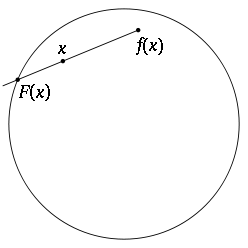
\includegraphics[scale=0.7]{sources/retraction_lemma}
\end{center}
\end{figure}
\end{proof}
We shall now prove the lemma.
\begin{proof}[of the lemma]
\begin{description}
\item[$n=1$:]
Define $\pi_0\prs{X} \ceq \set{\text{path connected componenets of $X$}}$.
A map $f \colon X \to Y$ which is continuous defines a map $\pi_0\prs{f} = f_{*} \colon \pi_0\prs{X} \to \pi_0\prs{Y}$ by $\brs{x} \mapsto \brs{f(x)}$ (this is well defined).
We observe that $\id_{*} = \id_{\pi_0\prs{X}}$.
Also, if $f \colon X \to Y$ and $g \colon Y \to Z$ then $\prs{g \circ f}_{*} = g_{*} f_{*}$.
Assume $r \colon \DD^1 \to \DD^1 = \SS^0$ is a retraction. We apply $\pi_0$ to
\[\
\begin{tikzcd}
\DD^1 \arrow[r, "r"] & \SS^0 \\
\SS^0 \arrow[u, "i", hook] \arrow[ru, "\id", swap] &
\end{tikzcd}
\]
and get the following diagram.
\[
\begin{tikzcd}
\pi_0\prs{\DD^1} \arrow[r, "r_*"] & \pi_0\prs{\SS^0} \\
\pi_0\prs{\SS^0} \arrow[u, "i_*"] \arrow[ru, "\id_* = \id", swap] &
\end{tikzcd}
\]

Now $\pi_0 \prs{\DD^1} = \text{singleton}$
and $\pi_0\prs{\SS^0} = \text{$2$ elements}$
contradicting the diagram.
\item[$n=2$:]
Let $\pi_1\prs{X,x_0}$ be the fundamental group. That is \[\pi_1\prs{X,x_0} = \pi_0\prs{\text{loops in $X$ that start and end in $x_0$}}\text{.}\]
Let $f \colon \prs{X, x_0} \to \prs{Y, y_0}$ be continuous (with $f\prs{x_0} = y_0$). This defines $\pi_1\prs{f} = f_{*} \colon \pi_1\prs{X,x_0} \to \pi_1\prs{Y,y_0}$.
It can be checked (and is showed in another topology course) that $\pi_1\prs{\DD^2, x} \cong 1$, and that $\pi_1\prs{\SS^1, x} \cong \Z$.
We get the following diagram, which gives a contradiction.

\[
\begin{tikzcd}
\pi_1\prs{\DD^2} \cong 1 \arrow[r, "r_*"] & \pi_1\prs{\SS^1} \cong \ZZ \\
\pi_1\prs{\SS^1} \cong \ZZ \arrow[u, "i_*"] \arrow[ru, "\id_* = \id", swap] &
\end{tikzcd}
\]

\end{description}
\end{proof}
We'd want to iterate such a construction by looking at loop spaces of loop spaces.\\
\begin{definition}
\[\pi_n = \pi_0 \prs{\text{loop of} \prs{\text{loop of} \ldots \prs{X, x_0} \tilde{x}_0, \ldots}}\]
\end{definition}
For $n \geq 1$, $\pi_n$ is a group. $\pi_1$ is a group with the operation of concatenation, and we can view $\pi_n$ as $\pi_1$ of some space, if $n \geq 1$. \\
We don't really like this inductive definition of $\pi_n$, so we'd like to give another definition. We can view $\pi_1$ as homotopy classes of $\prs{\SS^1, *} \to \prs{X, x_0}$. We'd like to generalise upon that idea. \\
\begin{definition}
$\pi_n$ is the group of homotopy classes of maps $\prs{\SS^n, *} \to \prs{X, x_0}$. We can view $\SS^n$ as $\quot{I^n}{\del I^n}$, and the group action of $\pi_n$ is given by gluing the spheres at the identified boundary of $\I^n$. It can be checked that $\pi_n$ is abelian for $n \geq 2$.
\end{definition}

\subsection{Homology and cohomology of topological spaces}
Homotopy groups are relatively difficult to compute. We'd want to introduce another algebraic object associate to topological spaces, $\tilde{H}_n$, which we shall see satisfies $\tilde{H}_n\prs{\SS^k} = \fcases{ 0 & n\neq k \\ \Z & n = k}$. We'll use this structure to prove Brouwer's theorem. \\
We define $H_0\prs{X} = \bigoplus_{\pi_0} \Z$ \stress{the zero'th homology group}, and similarly  $H_1\prs{X} = \pi_1\prs{X,x_0}^{\mathrm{ab}}$ \stress{the first homology group}.

\chapter{Simplicial Homology}
\section{$\Delta$-complexes}

\begin{definition}
Let $X$ be a topological space and $\sim$ be an equivalence relation on $X$.
The \stress{quotient space} is $\quot{X}{\sim}$. Let $\pi \colon X \to \quot{X}{\sim}$ be the projection, we say that $U \subseteq \quot{X}{\sim}$ is open in the quotient if and only if $\pi^{-1}\prs{U}$ is open in $X$.
\end{definition}
\begin{example}
We can construct the torus $\TT^2$ by gluing opposite sides of a square.
We write $X = \brs{0,1}^{2}$ and $\sim$ is the equivalence relation generated by $\prs{x,0} \sim \prs{x,1}$ and $\prs{0,y} \sim \prs{1,y}$.
%TODO fig. 2.1
\end{example}
\begin{example}
We can construct the Klein bottle $\KK^2$ by gluing opposite sides of a square, with one gluing in the opposite direction.
We write $X = \brs{0,1}^{2}$ and $\sim$ is the equivalence relation generated by $\prs{x,0} \sim \prs{x,1}$ and $\prs{0,y} \sim \prs{1,1-y}$.
%TODO fig. 2.2
\end{example}
\begin{example}
We can construct the \stress{real projective space} $\RR \mathrm{P}^n$ by \[\quot{\RR^{n+1}\setminus\set{0}}{\set{x \sim \lambda x}{\lambda \in \RR\setminus\set{0}}}\text{.}\]
%TODO fig. 2.3
\end{example}
\begin{definition}
Let $v_0, \ldots, v_n \in \RR^m$. We say $\set{v_i}_{i=1}^{n}$ are \stress{geometrically independent} if $\set{v_i - v_0}_{i=1}^n$ are linear-independent.
\end{definition}
\begin{example}
\begin{description}
\item[$n=0$:] Any point in $\RR^m$ is a $0$-simplex.
\item[$n=1$:] Any two \emph{distinct} points in $\RR^m$ are geometrically independent (we require $v_1 - v_0 \neq 0$). The convex hull is the segment connecting the points.
\item[$n=2$:] Geometrical independence means the three points aren't collinear.
\item[$n=3$:] Geometrical independence means the three points aren't coplanar, or equivalently that they span a full non-degenerate tetrahedron.
\end{description}
\end{example}
\begin{definition}
Given vectors $v_0, \ldots, v_n$, the \stress{convex hull} of the vectors is defined by the following.
\[\brs{v_0, \ldots, v_n} = \set{\sum_{i=0}^n t_i v_i}{\mat{t_i \geq 0 \\ \sum t_i = 1}}\]
\end{definition}
\begin{definition}
An \stress{$n$-simplex} is the convex hull of $n+1$ geometrically independent points in $\RR^m$.
\end{definition}
\begin{remark}
A simplex comes with an ordering of its vertices.
\end{remark}
\begin{definition}
Let $e_0, \ldots, e_n \in \RR^{n+1}$ be basis vectors.
$\brs{e_0, \ldots, e_n}$ is the \stress{standard $n$-simplex}.
%TODO fig 2.4
\end{definition}
\begin{definition}
The \stress{i\textsuperscript{th} face} of an $n$-simplex $\brs{v_0, \ldots, v_n}$ is defined by $\brs{v_0, \ldots, v_{i-1}, v_{i+1}, \ldots, v_n}$. We denote this by the following\footnote{The hat means we remove the vector $v_n$}. \[\brs{v_0, \ldots, \hat{v}_i, \ldots, v_n}\] 
\end{definition}
\begin{definition}
Let $v \in \brs{v_0, \ldots, v_n}$. It can be written as $\sum_{i=0}^n t_i v_i$ for $t_i \geq 0$ with $\sum t_i = 1$, \emph{uniquely}. $\prs{t_0, \ldots, t_n}$ are the \stress{barycentric coordinates}.
The inclusion map of the i\textsuperscript{th} face of $\brs{v_0, \ldots, v_n}$ in barycentric coordinates is
\[\iota_i \colon \prs{t_0, \ldots, t_{n-1}} \mapsto \prs{t_0, \ldots, t_{i-1}, 0, t_i, \ldots, t_{n-1}}\]
\end{definition}
\begin{definition}
We define the interior as \[\mathring{\Delta}^n = \Delta^n \setminus \text{faces of $\Delta^n$}\text{.}\]
\end{definition}
\begin{remark}
$\mathring{\Delta}^0 = \Delta^0$, because there are no faces.
\end{remark}
\begin{definition}
A \stress{$\Delta$-complex} structure on a topological space $X$ is a collection $\Sigma$ partitioned as \[\Sigma_n = \set{\text{set of $\sigma \colon \Delta^n \to X$ continuous}}\] such that the following properties hold.
\begin{enumerate}
\item For all $x\in X$ there's a unique $\sigma$ such that there's a unique $y \in \mathring{\Delta}^n$ with $x = \sigma\prs{y}$.\footnote{In words, every $x$ is the image of exactly one point in the interior of a face.}

\item For all $\sigma \in \Sigma_n$ and for all $0 \leq i \leq n$ there's $\tau \in \Sigma_{n-1}$ where $\sigma \circ \iota_i = \tau$.\footnote{In words, this means that restricting to a face, we keep the same ordering of the vertices. This defines an orientation on the complexes.}

\item $U \subseteq X$ is open if and only if $\sigma^{-1}\prs{U}$ is open for all $\sigma \in \Sigma$. This is called the \stress{CW topology}.
\end{enumerate}
\end{definition}
\begin{example}
See %TODO fig. 2.5
We have the following.
\[\Sigma = \set{\mat{
\Sigma_0 & v & \text{$0$-simplex} \\
\Sigma_1 & e_1, e_2, e_3 & \text{$1$-simplex} \\
\Sigma_2 & \sigma_1, \sigma_2 & \text{$2$-simplex}
}}\]
\end{example}
\begin{example}
See %TODO fig. 2.6 A
\end{example}
\begin{example}
See %TODO fig 2.6 B
this cannot be turned into a $\Delta$-simplex by addition of the diagonal. However, if we give a different direction to the edges as in %TODO fig 2.6 C
we can get a $\Delta$-simplex.
\end{example}
\begin{example}
The figure in %TODO fig. 2.7
is not a $\Delta$-simplex, because we cannot number the vertices in such a way that the direction of the arrows matches.
However, we can turn it into a simplex as in %fig. 2.9
\end{example}
\begin{example}
The Dunce hat in figure %TODO fig. 2.9
is a $\Delta$-complex.
\end{example}
\begin{definition}
Let $X$ have a $\Delta$-complex structure. The \stress{simplicial homology} on $X$ is the following.
\begin{align*}
C_i\prs{X} = \bigoplus_{\sigma \in \Sigma_i} \ZZ \sigma = \set{\sum_{j=1}^k n_j \sigma_j}{\mat{k \in \ZZ \\ n_j \in \ZZ \\ \sigma_j \in \Sigma_i}}
\end{align*}
where the sums are formal.
The elements of $C_i(X)$ are called \stress{$i$-chains}.
\end{definition}
\begin{definition}
The \stress{boundary map} on $X$ with a $\Delta$-complex structure is defined on $\sigma \in \Sigma_n$ by
\begin{align*}
\del_n \colon C_n\prs{X} &\to C_{n-1}\prs{X} \\
\sigma &\to \sum_{i=0}^n \prs{-1}^i \sigma \circ \iota_i
\end{align*}
and extended linearly to all maps.
\end{definition}
\begin{note}
We notice that $\del_0 = 0$.
\end{note}
\begin{example}
Let us calculate some boundary maps.
%TODO fig. 2.10
\end{example}
\begin{lemma}
$\del_{n-1} \circ \del_n = 0$.
\end{lemma}
\begin{proof}
\begin{align*}
\del_{n-1} \del_n \sigma &= \del_{n-1} \prs{\sum_{i=0}^n \prs{-1}^i \rest{\sigma}{\brs{v_0, \ldots, \hat{v}_i, \ldots, v_n}}} \\
&= \sum_{i=0}^n \prs{-1}^i \prs{\del_{n-1} \rest{\sigma}{\brs{v_0, \ldots, \hat{v}_i, \ldots, v_n}}} \\
&= \sum_{i=0}^n \prs{-1}^i \prs{\sum_{j < i} \prs{-1}^j \rest{\sigma}{\brs{v_0, \ldots, \hat{v}_j, \ldots, \hat{v}_i, \ldots, v_n}} + \sum_{i<j} \prs{-1}^{j-1} \rest{\sigma}{\brs{v_0, \ldots, \hat{v}_i, \ldots, \hat{v}_j, \ldots, v_n}}}
\end{align*}
The coefficient of $\rest{\sigma}{\brs{v_0, \ldots, \hat{v}_i, \ldots, \hat{v}_j, \ldots, v_n}}$ is $\prs{-1}^i\prs{-1}^{j-1} + \prs{-1}^j \prs{-1}^i = 0$.
\end{proof}
\begin{definition}
A sequence of abelian groups
\[\ldots \rightarrow C_n\prs{X} \xrightarrow{\del_n} C_{n-1}\prs{X} \rightarrow \ldots\]
with $\del_{n-1} \circ \del_n = 0$
is called a \stress{chain complex}.
\end{definition}
\begin{exercise}
Calculate $\del_0 \del_1$ of a line and $\del_1 \del_2$ of a triangle.
\end{exercise}
\begin{remark}
Because the $n$ in $\del_n$ is clear from the domain and codomain, we sometimes write $\del$ instead of $\del_n$.
\end{remark}
\begin{remark}
$\del_n \circ \del_{n+1} = 0$ implies $\im \del_{n+1} \subseteq \ker \del_n$.
\end{remark}
\begin{definition}
\stress{The n\textsuperscript{th} homology} is
\[H_n\prs{X} \ceq \quot{\ker \del_n}{\im \del_{n+1}} \text{.}\]
Similarly we can write $H_n\prs{X,A}$ where $C_n\prs{X}$ is an $A$-span of $\Sigma_n$, $A$ being any abelian group instead of $\ZZ$.
\end{definition}
\begin{definition}
The elements of $\ker\prs{\del_n} \eqqcolon Z_n$ are called \stress{cycles}.\\
The images of $\im\prs{\del_{n+1}} \eqqcolon B_n$ are called \stress{boundaries}.\\
The elements of $H_n\prs{X}$ are called \stress{homoloy classes}.\\
If $x,y \in Z_n$ and $\brs{x} = \brs{y} \in H_n\prs{X}$, then $x$ and $y$ are called \stress{homologous}.
\end{definition}
\begin{example}
Take $X = \SS^1$ with the $\Delta$-complex structure in figure \ref{circle delta complex}.
\begin{figure}[!tpb]
%TODO AT 3.1
\caption{Circle $\Delta$ complex.}
\label{circle delta complex}
\end{figure}
We have $\del(e) = v$ and therefore the following chain.
\[
\begin{tikzcd}
\ldots \arrow[r] & C_3 \arrow[r] & C_2\prs{\SS^1} \arrow[r] & C_1\prs{\SS^1} \arrow[r] & C_0\prs{\SS^1}  \arrow[r] & 0 \arrow[r] & 0 \arrow[r] & \ldots \\
\ldots \arrow[r, "0"] & 0 \arrow[r, "0"] &  0 \arrow[r, "0"]  & \ZZ e \arrow[r, "0"] & \ZZ v \arrow[r, "0"] &  0 \arrow[r, "0"] & 0 \arrow[r, "0"]  & \ldots
\end{tikzcd}
\] %TODO fill equalities

Computing the homologies, we have
\begin{align*}
H_0\prs{\SS^1} \quot{\ZZ r}{0} \cong \ZZ \\
H_1\prs{\SS^1} = \quot{\ZZ e}{0} \cong \ZZ \\
\forall k \geq 1 \colon H_k\prs{\SS^1} = 0
\end{align*}
\end{example}
\begin{example}
Take $X$ to be as in %TODO fig AT 3.2
We $\del\prs{e_i} = w-v$, and the following chain.
\[
\begin{tikzcd}
\ldots \arrow[r] &  C_3 \arrow[r] & C_2\prs{X} \arrow[r] & C_1\prs{X} \arrow[r] & \arrow[r] C_0\prs{X}  \arrow[r] & 0 \arrow[r] & 0 \arrow[r] & \ldots \\
\ldots \arrow[r, "0"] & 0 \arrow[r, "0"] & 0 \arrow[r, "0"]  & \ZZ e_1 \oplus \ZZ e_2 \oplus \ZZ e_3 \arrow[r, "\del"] & \ZZ v \oplus \ZZ w \arrow[r, "0"] &  0 \arrow[r, "0"]  & 0 \arrow[r, "0"] & \ldots
\end{tikzcd}
\] %TODO fill equalities
Computing $H_0$ we have
\[H_0 \prs{X} = \quot{\ZZ v \oplus \ZZ w}{\trs{w-v}} \cong \ZZ\brs{v}\]
because in the quotient $w=v$.\\
Computing $H_1$ we have
\[H(X) = \quot{\ker \del}{\cancel{\im}} \cong \ker \del = \trs{e_1 - e_2, e_2 - e_3}\text{.}\]
Then $\ker\del = \set{a_1 e_1 + a_2 e_2 + a_3 e_3}{a_1 + a_2 + a_3 = 0}$.
We have that for all $k \geq 2$, $H_k\prs{X} = 0$.
\end{example}
\begin{remark}
$H_0$ "counts the number of connected components",
$H_1$ "counts the number of holes", et cetera.
\end{remark}
\begin{example}
Take $\TT^2$ as in %TODO fig AT 3.3
We have the following chain
\[
\begin{tikzcd}
\ldots \arrow[r] &  C_3 \arrow[r] & C_2\prs{X} \arrow[r] & C_1\prs{X} \arrow[r] & \arrow[r] C_0\prs{X}  \arrow[r] & 0 \arrow[r] & 0 \arrow[r] & \ldots \\
\ldots \arrow[r, "0"] & 0 \arrow[r, "0"] & \ZZ \sigma_1 \oplus \ZZ \sigma_2 \arrow[r, "\del_2"]  & \ZZ e_1 \oplus \ZZ e_2 \oplus \ZZ e_3 \arrow[r, "0"] & \ZZ v \arrow[r, "0"] &  0 \arrow[r, "0"]  & 0 \arrow[r, "0"] & \ldots
\end{tikzcd}
\] %TODO fill equalities
with
$\del_2\prs{\sigma_1} = e_2 + e_1 - e_3$ and $\del_2\prs{\sigma_2} = e_1 + e_2 - e_3$.
We have 
\begin{align*}
H_0(X) &\cong \ZZ v \\ H_1(X) &\cong \quot{\ZZ e_1 \oplus \ZZ e_2 \oplus \ZZ e_3}{\trs{e_1 + e_2 - e_3}} = \quot{\trs{e_1,e_2,e_3}}{e_3 = e_1 + e_2} \cong \trs{e_1, e_2} \cong \ZZ^2 \\ H_2(X) &\cong \ker \del_2 = \trs{\sigma_1 - \sigma_2} \cong \ZZ\trs{\sigma_1 - \sigma_2} \text{.}
\end{align*}
\end{example}
\begin{example}
Take $\RR\P^2$ as in %TODO fig AT 3.4
We have the chain \[\trs{\sigma_1, \sigma_2} \to \trs{e_1, e_2, e_3} \to \ZZ r \oplus \ZZ w \xrightarrow{0} 0\]
with maps
\begin{align*}
e_1 \mapsto w-v \\ e_2 \mapsto w-v \\ e_3 \mapsto 0
\end{align*}
and
\begin{align*}
\sigma_1 \mapsto e_3 + e_1 - e_2 \\
\sigma_2 \mapsto e_3 + e_2 - e_1\text{.}
\end{align*}
Computing homologies we get that following.
\begin{align*}
H_0 &\cong \ZZ\brs{v} \\
H_1 &= \quot{\trs{e_3, e_1 - e_2}}{\trs{\beta - \alpha, \beta + \alpha}} \cong \quot{\ZZ\alpha}{2\alpha} \cong \quot{\ZZ}{2\ZZ} \quad \alpha \ceq e_1 - e_2, \beta = e_3 \\
H_2 &= \ker\del_2 = a_1 \sigma_1 + a_2\sigma_2 = 0 \text{.}
\end{align*}
\end{example}
\begin{example}
Take $X = \SS^n$.
We can write the sphere as a result of gluing two discs of lower dimension.
\[\SS^n = \DD^n \underset{\del \DD^n \equiv \del \DD^n}{\amalg} \DD^n\]
Therefore we write \[\SS^n = \overset{\sigma_1}{\overbrace{\Delta^n}} \underset{\del \Delta^n \equiv \del \Delta^n}{\amalg} \overset{\sigma_2}{\overbrace{\Delta^n}} \text{.}\]
The n\textsuperscript{th} homology is $H_n\prs{\SS^n} = \quot{\ker \del_n}{\cancel{\im \del_{n+1}}}$.
We have $C_{n+1} = 0$, $C_n = \ZZ \sigma_1 \oplus \ZZ \sigma_2$ and the relation $\del_n \sigma_1 = \del_n \sigma_2$. Therefore
\[\ker \del_n = \trs{\sigma_1 - \sigma_2} \cong \ZZ\]
which brings
$H_n\prs{\SS^n} \cong \ZZ$.
\end{example}
\begin{remark}
The homology we have so far defined is called \stress{simplicial homology}. We sometimes write $H_n^{\Delta}\prs{X}$ to note that. We shall define also \stress{singular homology}, and later we show that these are equivalent.
\end{remark}
\section{Singular Homology}
\begin{definition}
Let $X$ be a topological space, and let \[\Sigma_n^{\mrm{sing}} = \set{\sigma \colon \Delta^n \to X}{\text{$\sigma$ is continuous}}\text{.}\]
$\sigma \in \Sigma_n^{\mrm{sing}}$ is called a \stress{singular simplex}.
$C_i^{\mrm{sing}} \ceq \bigoplus_{\Sigma_i} \ZZ$ is an \stress{$i$-chain}.
$\del_n \colon C_n^{\mrm{sing}} \to C_{n-1}^{\mrm{sing}}$ are defined as before and satisfy $\del_{n-1}\circ \del_n = 0$. We obtain a chain
\[\ldots \to C_n^{\mrm{sing}}\prs{X} \to C_{n-1}^{\mrm{sing}}\prs{X} \to \ldots \to C_0^{\mrm{sing}}\prs{X} \to 0\]
and define the \stress{singular homology}
$H_n^{\mrm{sing}}\prs{X} = \quot{\ker \del_n}{\im \del_{n+1}}$.
\end{definition}
\begin{remark}
We may not write $\mrm{sing}$, but understand that the following computations are done in singular homology. 
\end{remark}
\begin{lemma}
Let $X = \set{x}$. Then $H_n\prs{X} = \fcases{\ZZ & n=0 \\ 0 & n>0}$.
\end{lemma}
\begin{proof}
Note that $\Sigma_n = \set{\sigma^n_{\mrm{const}}}$ for $n \geq 0$.
We have $C_i(X) = \ZZ \sigma^i_{\mrm{const}}$ and the following chain.
\[\ldots \to \ZZ \sigma^3_{\mrm{const}} \to \ZZ \sigma^2_{\mrm{const}} \to \ZZ \sigma^1_{\mrm{const}} \to \ZZ \sigma^0_{\mrm{const}} \to 0\]
Now \[\del_n\prs{\sigma^n_{\mrm{const}}} = \sum_{i=0}^n \prs{-1}^i \sigma_{\mrm{const}}^{i}\]
so $\del_n$ is the zero map where $n$ is odd, and an isomorphism if $n$ is even.
Looking at the kernel and image gives $H_0 = \ZZ$ and $H_i = 0$ for all $i \geq 1$.
\end{proof}

\begin{remark}
A map $f \colon X \to Y$ induces a map $\Sigma_n(X) \to \Sigma_n(Y)$ by $\sigma \mapsto f\circ \sigma$. This extends linearly to a map
\[f_{\#} \colon C_n\prs{X} \to C_n\prs{Y}\text{.}\]
\end{remark}
\begin{definition}
If we look at $g$ as a map between $\prs{C_n(X)}_{n\in\NN}$ and $\prs{C_n(Y)}_{n\in\NN}$, and the following commutes, and we call $g$ a \stress{chain map}.
\[
\begin{tikzcd}
\ldots \arrow[r] & C_{n+1}(X) \arrow[d,"g"] \arrow[r,"\del"] & C_{n}(X) \arrow[r,"\del"] \arrow[d,"g"] & C_{n-1}(X) \arrow[r,"\del"] \arrow[d,"g"] & \ldots \\
\ldots \arrow[r] & C_{n+1}(Y) \arrow[r,"\del"] & C_{n}(Y) \arrow[r,"\del"] & C_{n-1}(Y) \arrow[r,"\del"] & \ldots
\end{tikzcd}
\]
\end{definition}
\begin{claim}
$f_{\#}$ is a chain map.
\end{claim}
\begin{proof}
\begin{align*}
f_{\#}\prs{\del \sigma} &= f_{\#}\prs{\sum_{i=1}^n \prs{-1}^i \rest{\sigma}{\brs{v_0, \ldots, \hat{v}_i, \ldots, v_n}}} \\
&= \sum_{i=0}^n \prs{-1}^i \rest{\prs{f\circ\sigma}}{\brs{v_0, \ldots, \hat{v}_i, \ldots, v_n}} \\
&= \del \prs{f_{\#}\prs{\sigma}}
\end{align*}
\end{proof}
\begin{corollary}
$f_{\#}$ is a chain map, therefore it induces a map $f_{*} \colon H_n\prs{X} \to H_n\prs{Y}$.
\end{corollary}
\begin{claim}
$f_*$ is well defined.
\end{claim}
\begin{proof}
$H_n\prs{X} = \quot{Z_n\prs{X}}{B_n\prs{X}}$.
If $z \in Z_n\prs{X}$, then $f_{\#}\prs{z} \in Z_n\prs{Y}$ and
\[\del f_{\#}z = f_{\#}\del z \stackrel[z \in Z_n\prs{X}]{}{=} f_{\#} 0 = 0\text{.}\]
So, have $f_{\#} \colon Z_n(X) \to Z_n(Y)$
by
$\brs{z} \mapsto \brs{f_{\#}(z)}$. \\
If $b \in B_n\prs{X}$, then $f_{\#}b \in B_n\prs{Y}$ and there's $p \in C_n\prs{X}$ such that $b = \del p$.
Now
\[\del f_{\#}\prs{p} = f_{\#}\prs{\del p} = f_{\#}\prs{b}\text{.}\]
\end{proof}
\begin{remark}
\begin{enumerate}
\item $\prs{f \circ g}_{*} = f_{*} \circ g_{*}$. This is true because it's true for $\prs{f \circ g}_{\#}$, and by definition of $\prs{f \circ g}_{*}$.
\item $\prs{\id_X}_{*} = \id_{H\prs{X}}$.
\end{enumerate}
\end{remark}
\begin{corollary}
$X\cong Y$ implies $H_{i}(X) \cong H_{i}(X)$ for all $i$.
\end{corollary}
\begin{definition}
Let $f,g \colon X \to Y$ be continuous between topological spaces.
We call $f,g$ \stress{homotopic} if there's a map
\[h \colon X \times \brs{0,1} \to Y\]
such that $\rest{h}{X \times \set{0}} = f$ and $\rest{h}{X \times \set{1}} = g$.
We write $f \approx x$ or $f \cong g$.
\end{definition}
\begin{definition}
Let $X,Y$ be topological. They're called \stress{homotopy equivalent} if there's $f \colon X \to Y$ and $g \colon Y \to X$ such that $g \circ f \approx \id_X$ and $f \circ g \approx \id_Y$.
\end{definition}
\begin{proposition}
If $f,g \colon X \to Y$ and $f \approx g$, then $f_{*} = g_{*}$.
\end{proposition}
\begin{corollary}
If $X \approx Y$ are homotopy equivalent, then $H_i(X) \cong H_i\prs{Y}$ for all $i$.
\end{corollary}
\begin{proof}
The following commutes in homotopy.
\[
\begin{tikzcd}
X \arrow[r,"f"] \arrow[rr,bend right=60, "\id"] & Y \arrow[r,"g"] & X
\end{tikzcd}
\]
So, applying $\prs{}_{*}$ we get
\[g_{*} \circ f_{*} = \prs{g\circ f}_{*} = \id_{*} = \id\text{.}\]
\end{proof}
\begin{definition}
$X$ is \stress{contractible} if $X \approx *$.
\end{definition}
\begin{corollary}
$H_n\prs{X} = \fcases{ \ZZ & n=0 \\ 0 & n > 0}$ for $X$ contractible.
\end{corollary}
\begin{proof}[of the proposition]
We want to construct maps $P \colon C_n\prs{X} \to C_{n+1}\prs{Y}$ such that $\del P = g_{\#} - f_{\#} - P\del$.
Then the following commutes.
\[
\begin{tikzcd}
\ldots \arrow[r] & C_n\prs{X} \arrow[r] \arrow[dl, "P_{n}", swap] \arrow[d,"f_{\#}", shift left = 1]\arrow[d,"g_{\#}", swap, shift right = 1]& C_{n-1}(X) \arrow[r] \arrow[dl, "P_{n-1}", swap] \arrow[d,"f_{\#}", shift left = 1]\arrow[d,"g_{\#}", swap, shift right = 1] & \ldots \\
\ldots \arrow[r] & C_n\prs{Y} \arrow[r] & C_{n-1}(Y) \arrow[r] & \ldots
\end{tikzcd}
\]
We obtain that for $z \in Z_n\prs{X}$
\[g_{\#}\prs{z} - f_{\#}\prs{z} = \del P\prs{z} + P\underset{=0}{\underbrace{\del\prs{z}}} \in B_n\prs{Y}\]
then
$g_{*} - f_{*} = 0 \in H_n\prs{Y}$
and then $g_{*} = f_{*}$.\\
Define \[P\prs{\sigma} = \sum_{i=0}^n \prs{-1}^i \rest{h \circ \prs{\sigma \times \id}}{\brs{v_0, \ldots, v_i, w_i, w_n}}\text{.}\]
See figures \ref{prism_map} and \ref{prism:examples}.
\begin{figure}[!tbp]
\caption{Prism map.}
\label{prism_map}
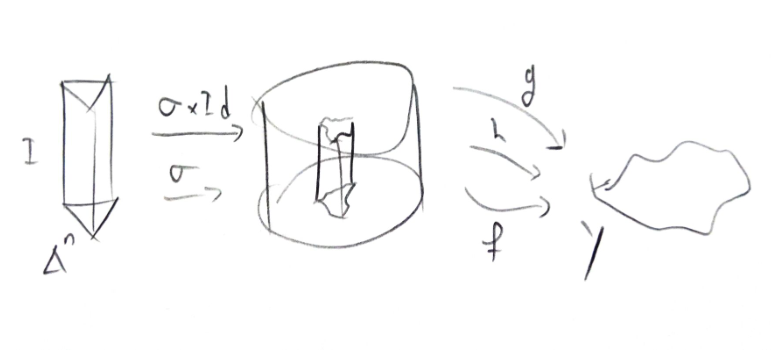
\includegraphics[scale=0.8]{sources/prism1}
\end{figure}

\begin{figure}[!tbp]
  \begin{subfigure}[b]{0.4\textwidth}
    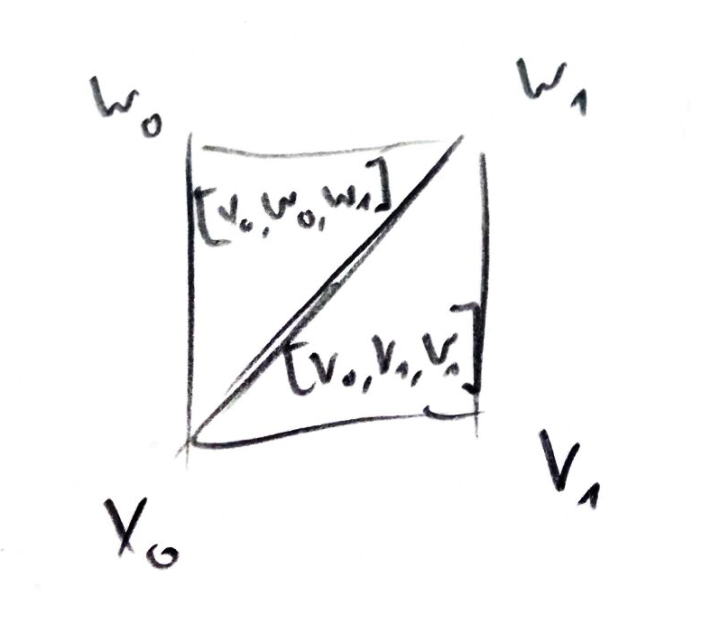
\includegraphics[width=\textwidth]{sources/prism2}
    \caption{Prism one.}
    \label{fig:f1}
  \end{subfigure}
  \hfill
  \begin{subfigure}[b]{0.4\textwidth}
    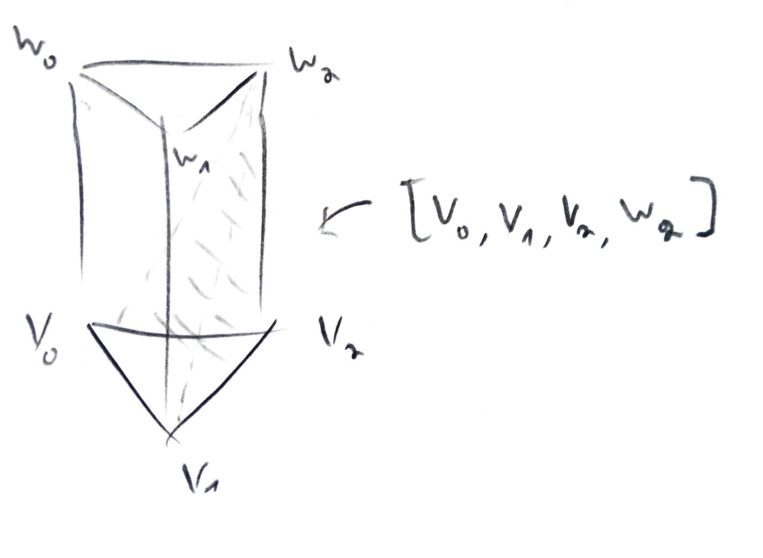
\includegraphics[width=\textwidth]{sources/prism3}
    \caption{Prism two.}
    \label{fig:f2}
  \end{subfigure}
  \caption{Prism examples.}
  \label{prism:examples}
\end{figure}

We have the following
\begin{align*}
\del P\prs{\sigma} &= \sum_{0 \leq j \leq i \leq n} \prs{-1}^i \prs{-1}^j h \circ \rest{\prs{\sigma \times \id}}{\brs{v_0, \ldots, \hat{v}_j, \ldots, v_i, w_i, \ldots, w_n}} \\&+ \sum_{0 \leq i \leq j \leq n} \prs{-1}^i \prs{-1}^{j+1} h \circ \rest{\prs{\sigma \times \id}}{\brs{v_0, \ldots, v_i, w_i, \ldots, \hat{w}_j, \ldots, w_n}}
\end{align*}
Looking at $i=j=k$ we have in the first sum \[\cancel{\prs{-1}^i \prs{-1}^j} h\circ\rest{\prs{\sigma \times \id}}{\brs{v_0, \ldots, v_{k-1},w_k, \ldots, w_n}}\text{.}\]
Looking at the second sum where $i=j=k-1$ we get
\[\cancel{\prs{-1}^{k-1}\prs{-1}^k} h\circ\rest{\prs{\sigma \times \id}}{\brs{v_0, \ldots, v_{k-1},w_k, \ldots, w_n}}\text{.}\]
Therefore these cancel out. Among $i=j$ summands we are left with
\begin{align*}
&\overset{g_{\#}\sigma}{\overbrace{{\prs{-1}^0\prs{-1}^0} h\circ\rest{\prs{\sigma \times \id}}{\brs{w_0, \ldots, w_n}}}} \\&+ 
\overset{f_{\#}\sigma}{\overbrace{\prs{-1}^{n} \prs{-1}^{n+1} h \circ \rest{\prs{\sigma \times \id}}{\brs{v_0, \ldots, v_n}}}}\text{.}
\end{align*}
Computing $P\del \prs{\sigma}$ we get the following.
\begin{align*}
P \del \prs{\sigma} &= P\prs{\sum_{i=1}^n \prs{-1}^i \rest{\sigma}{\brs{v_0, \ldots, \hat{v}_i, \ldots, v_n}}} \\ &=
\sum_{j < i} \prs{-1}^i \prs{-1}^j h\circ \rest{h \circ \prs{\sigma \times \id}}{\brs{v_0, \ldots, v_j, w_j, \ldots, \hat{w}_i, \ldots, w_n}} \\&+
\sum_{i<j} \prs{-1}^i \prs{-1}^{j-1} \rest{h\circ \prs{\sigma \times \id}}{\brs{v_0, \ldots, \hat{v}_i, \ldots, v_j, w_j, \ldots, w_n}} \\&= \del P - \prs{g_{\#} - f_{\#}}
\end{align*}
So, $P$ satisfies the required property.
\end{proof}
\begin{definition}
A map $H \colon X\times\brs{0,1} \to X$ is an \stress{isotopy} if $H\prs{\cdot,t}$ are all homeomorphisms.
\end{definition}
\begin{proposition}
If $X\neq \ns$ is path-connected, then $H_0\prs{X} \cong \ZZ$.
\end{proposition}
\begin{proof}
Examine the chain complex
\[C_2(X) \xrightarrow{\del} C_1(X) \xrightarrow{\del} C_0(X) \rightarrow 0\text{.}\]
Let $\eps \colon C_0\prs{X} \to \ZZ$ be the map defined by $v \mapsto 1$ for $v \in \Sigma_0$. Then
\[\sum \alpha_v v \mapsto \sum \alpha_v \text{.}\]
We want to show that $\ker \eps = \im \del_1$.
\begin{description}
\item[$\supseteq$:]
Let $e \in \Sigma_1$ be viewed as $e \colon \brs{v_0, v_1} \to X$. So,
\[\eps \prs{\del e} = \eps \prs{\rest{e}{v_1} - \rest{e}{v_0}} = 1-1 = 0 \text{.}\]
\begin{remark}
\[\ldots \xrightarrow{\del} C_1\prs{X} \xrightarrow{\del} C_0\prs{X} \xrightarrow{\eps} \ZZ \to 0\]
is a chain complex. The homology of this chain complex is called the \stress{reduced (singular) homology of $X$} and is denoted $\tilde{H}_i\prs{X}$. Note that $\tilde{H}_i\prs{X} = H_i\prs{X}$ for all $i \geq 1$.
\end{remark}
\item[$\subseteq$:]
Let $\sum \alpha_v v \in \ker \eps$. I.e. $\sum \alpha_v = 0$.\\
Let $v_0 \in \Sigma_0$. Let $e_v$ be a path (i.e. a 1-simplex) from $v_0$ to $v$. Let $\lambda = \sum \alpha_v e_v \in C_1\prs{X}$.
Now
\[\del \lambda = \sum \alpha_v\prs{v-v_0} = \sum \alpha_v v - \overset{=0}{\overbrace{\prs{\sum \alpha_v}}} v = \sum \alpha_v v \text{.}\]
\end{description}
\end{proof}
\begin{proposition}[home-work]
If $\set{C_i}_{i \in A}$ are the path-connected components of $X$ then $H_n\prs{X} = \bigoplus_{i \in A} H_n\prs{C_i}$.
\end{proposition}
\begin{corollary}
$H_0\prs{X} = \oplus_{i \in A} \ZZ$.
\end{corollary}
Examine $\sum \alpha_e e \in Z_1$. We can form a space by pairing to get $\sum \alpha_e' e \in Z$ with $\alpha_e' \in \set{\pm 1}$ where the sum is taken with repetitions.
Now
$\del \prs{\sum \alpha_e e} = 0$. Take a disjoint union of such intervals and glue their boundaries according to the pairing.
For example in \eqref{simplex:pairing}
\begin{figure}[!tbp]
  \begin{subfigure}[b]{0.4\textwidth}
    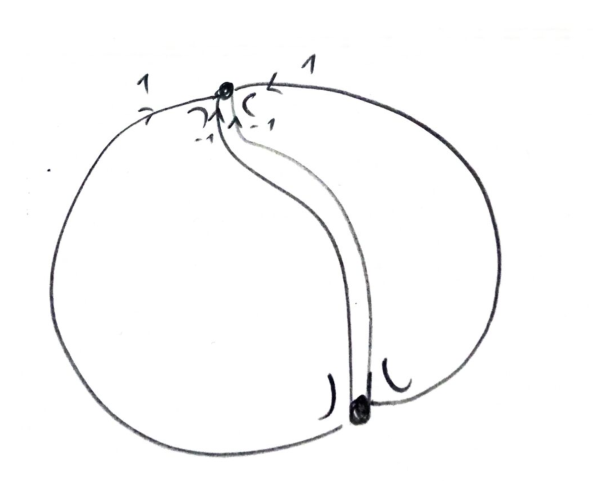
\includegraphics[width=\textwidth]{sources/4_1a}
  \end{subfigure}
  \hfill
  \begin{subfigure}[b]{0.4\textwidth}
    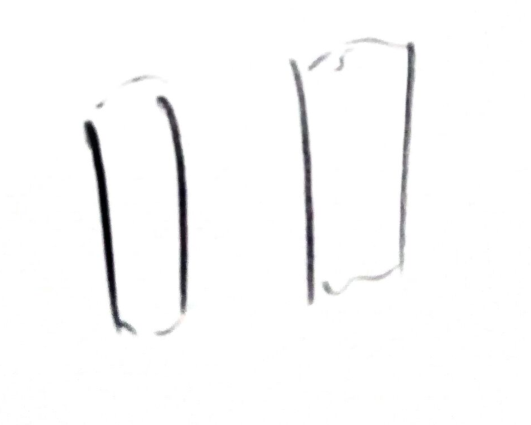
\includegraphics[width=\textwidth]{sources/4_1b}
  \end{subfigure}
  \caption{Simplex pairing.}
  \label{simplex:pairing}
\end{figure}
we get two circles and in \eqref{simplex:pairing2}.
\begin{figure}[!tbp]
  \begin{subfigure}[b]{0.4\textwidth}
    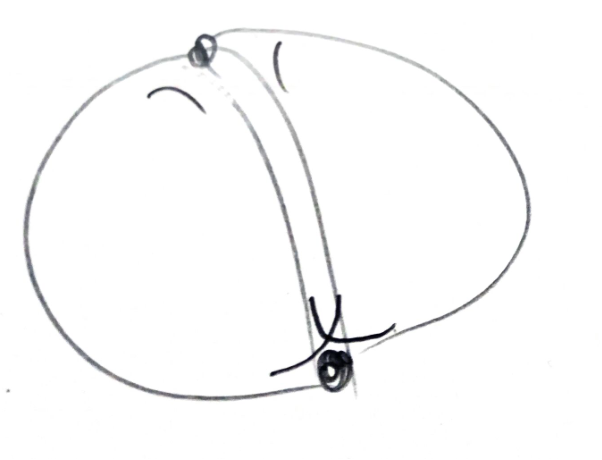
\includegraphics[width=\textwidth]{sources/4_2a}
  \end{subfigure}
  \hfill
  \begin{subfigure}[b]{0.4\textwidth}
    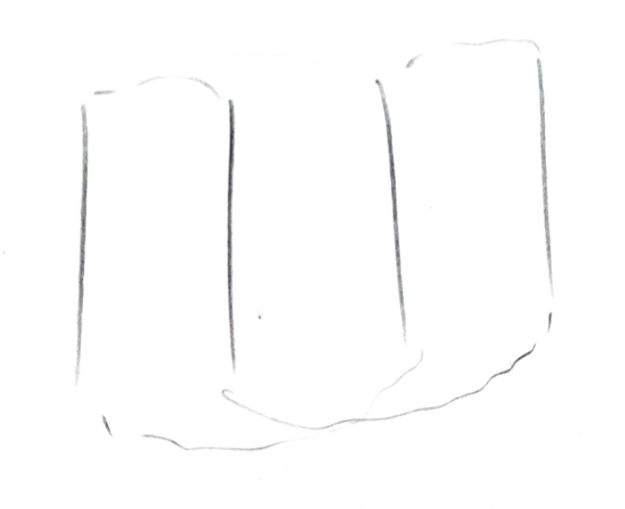
\includegraphics[width=\textwidth]{sources/4_2b}
  \end{subfigure}
  \caption{More simplex pairing.}
  \label{simplex:pairing2}
\end{figure}
we get one.
By gluing in such a way we obtain a one-dimensional topological manifold.

\begin{definition}
A \stress{topological manifold} is a space $X$ (Hausdorff, second countable) which is locally homeomorphic to $\RR^n$. 
\end{definition}
\begin{remark}
$1$-manifolds are $\RR$ and $\SS^1$, so as the above construction gives a compact space, we obtain a disjoint union of circles.
\end{remark}

We can similarly repeat such a construction for $Z_2$.

\begin{remark}
The important property of the construction is that \emph{every face ($\mrm{codim}=1$) appears in exactly $2$ pairs of $n$-simplices and faces.}
\end{remark}
\begin{remark}
Take $\lambda \in C_2\prs{X}$, we can view it as a $2$-manifold with a surface. Then, taking a complex on the surface, the boundary map is trivial on inner edges, and is non-trivial on the boundary.
See figure \eqref{manifold:boundary}.
\begin{figure}
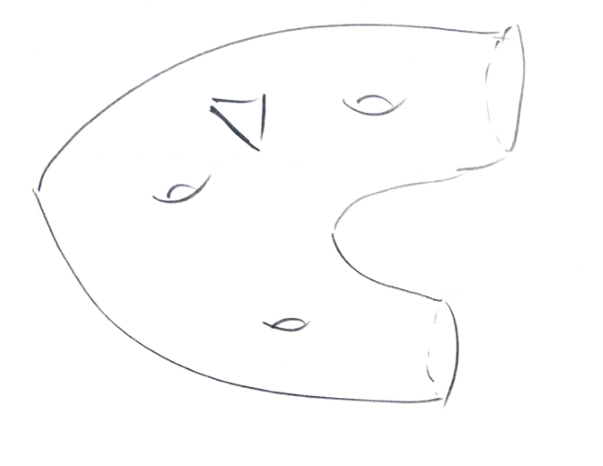
\includegraphics[scale=0.7]{sources/4_3}
\caption{Manifold with boundary}
\label{manifold:boundary}
\end{figure}
\end{remark}

Our current \emph{goal} is to relate homologies of $X$ and $A \subseteq X$ to the homology of $\quot{X}{A}$.

\section{Exact sequences}
\begin{definition}
The sequence
\[\ldots \rightarrow A \xrightarrow{\alpha} B \xrightarrow{\beta} C \xrightarrow \ldots\]
is said to be \stress{exact at $B$} if $\ker \beta = \im \alpha$.
The sequence is \stress{exact} if it's exact at all objects.
\end{definition}
\begin{example}
$0 \to A \xrightarrow{\alpha} B$ is exact if and only if $\alpha$ is injective.
\end{example}
\begin{example}
$B \xrightarrow{\beta} C \to 0$ is exact if and only if $\beta$ is surjective.
\end{example}
\begin{example}
$0 \to A \xrightarrow{\alpha} B \to 0$ is exact if and only if
$\alpha$ is surjective.
\end{example}
\begin{definition}
A \stress{short exact sequence} is of the form
\[0 \to A \xrightarrow{\alpha} B \xrightarrow{\beta} C \to 0\text{.}\]
\end{definition}
\begin{remark}
From the isomorphism theorem, such a short exact sequence, $\beta$ induces an isomorphism
\[C \stackrel[\beta]{}{\cong} \quot{B}{\alpha\prs{A}}\text{.}\]
We have $A \xhookrightarrow{\alpha} B$ so we may write $C \cong \quot{B}{A}$.
\end{remark}
\begin{definition}
Let $A \subseteq X$ be topological spaces. $X$ \stress{deformation retracts to} $A$ if there's $h \colon X \times \brs{0,1} \to X$ such that the following hold.
\begin{align*}
\rest{h}{X \times \set{0}} &= \id_X \\
h\prs{X \times \set{1}} &\subseteq A \\
\forall a \in A \colon h\prs{a,t} &= a
\end{align*}
\end{definition}
\begin{example}
$\SS^{n-1}$ is a deformation retract of $\RR^n \setminus \set{0}$. Take \[h\prs{v,t} = \prs{1-t + \frac{t}{\norm{v}}}v\text{.}\]
\end{example}
\begin{theorem}
Let $X$ be a topological space and $A \subseteq X$ non-empty, closed, and a deformation retract of an open neighbourhood $V \supseteq A$. Then there is a long exact sequence
\[\tilde{H}_n\prs{A}\xrightarrow{i_{*}} \tilde{H}_n\prs{X} \xrightarrow{q_*} \tilde{H}_n \prs{\quot{X}{A}} \xrightarrow{\del} \tilde{H}{n-1} \prs{A} \to \ldots \to \tilde{H}_0 \prs{\quot{X}{A}} \to 0 \text{.}\]
This $\del$ isn't the boundary map on chains, but a different boundary map we shall construct. $i \colon A \to X$ is the inclusion and $q \colon X \to \quot{X}{A}$ is the quotient map. 
\end{theorem}
\begin{corollary}[homologies of $\SS^n$]
\[\tilde{H}_n\prs{\SS^n} = \fcases{\ZZ & n=k \\ 0 & n\neq k}\]
\end{corollary}
\begin{proof}
By induction on $n$.
\begin{description}
\item[Basis, $n=0$:]
We have $\SS^0 = \set{p_1, p_2}$. Then \[\tilde{H}_n\prs{\SS^0} = \fcases{\ZZ & k=0 \\ 0 & k\neq 0}\]
because
\[H_k\prs{\SS^0} = \fcases{\ZZ^2 & k=0 \\ 0 & k\neq 0}\]
and
\begin{align*}
H_k = \fcases{\tilde{H}_k & k > 0 \\ \tilde{H}_k \oplus \ZZ & k > 0}\text{.}
\end{align*}
\item[Step, $n > 0$:]
Note that $\SS^n = \quot{\DD^n}{\del \DD^n}$ and $\del \DD^n = \SS^{n-1}$.
Also, $\del \DD^n = \SS^{n-1}$ and $\DD^n$ satisfy the assumption of the theorem.
We obtain the following.
\begin{align*}
\ldots \rightarrow \tilde{H}_k \prs{\del \DD^n} \to \tilde{H}_k \prs{\DD^n} \to \tilde{H}_k \prs{\quot{\DD^n}{\del \DD^n}} \to \tilde{H}_{k-1}\prs{\del \DD^n} \to\tilde{H}_{k-1}\prs{\del{\DD^n}} \to \ldots
\end{align*}
From homework, $\DD^n$ is contractible so $\tilde{\H}_k\prs{\DD^n} = 0$ for all $k$. Hence we get the following
\begin{align*}
\ldots \rightarrow \tilde{H}_k \prs{\del \DD^n} \to \cancelto{0}{\tilde{H}_k \prs{\DD^n}} \to \tilde{H}_k \prs{\quot{\DD^n}{\del \DD^n}} \to \tilde{H}_{k-1}\prs{\del \DD^n} \to\cancelto{0}{\tilde{H}_{k-1}\prs{\del{\DD^n}}} \to \ldots
\end{align*}
so
\[\tilde{H}_k \prs{\quot{\DD^n}{\del \DD^n}} \cong \tilde{H}_{k-1} \prs{\del \DD^n} \stackrel[\text{induction}]{}{\cong} \fcases{ \ZZ & n=k \\ 0 & n \neq k} \text{.}\]
\end{description}
\end{proof}
\begin{definition}
Let $A \subseteq X$ be topological spaces. We call $\prs{X,A}$ a \stress{pair of spaces}.
A map $f \colon \prs{X,A} \to \prs{Y,B}$ is \stress{a (continuous) map between pairs} if $f \colon X \to Y$ is continuous such that $f\prs{A} \subseteq B$.
\end{definition}
\begin{remark}
$A \xhookrightarrow{i} X$ induces a map $C_n\prs{A} \xhookrightarrow{i_{\#}} C_n\prs{X}$. We denote $C_n\prs{A} \subseteq C_n\prs{X}$.
\end{remark}
\begin{definition}
The \stress{relative chains} are
\[C_n\prs{X,A} \ceq \quot{C_n\prs{X}}{C_n\prs{A}}\text{.}\]
\end{definition}
\begin{remark}
Note that $\del C_n\prs{A} \subseteq C_{n-1}\prs{A}$ where $\del$ is the boundary map of $X$.\\
$\del$ induces a map
\[\del \colon C_n\prs{X, A} \to C_{n-1} \prs{X,A}\text{.}\]
\end{remark}
\begin{remark}
$\del^2 = 0$ for $C_n\prs{X}$ therefore $\del^2 = 0$ for $C_n\prs{X,A}$ (for we take a quotient of zero).
\end{remark}
\begin{definition}
\[C_n\prs{X,A} \xrightarrow{\del} C_{n-1}\prs{X,A} \to \ldots\]
is the \stress{relative chain complex}.
\end{definition}
\begin{definition}
$H_n\prs{X,A}$, the homologies of the relative chain complex, are the \stress{relative homologies of $\prs{X,A}$}.
\end{definition}
\begin{example}
A relative cycle happens to match a manifold in $X$ that may have a boundary, only in $A$. I.e. after identifying the points of $A$, we the manifold wouldn't have a boundary. %TODO fig AT 5.1
\end{example}
\begin{example}
A relative boundary is a boundary of a manifold after identifying the points on $A$. %TODO fig AT 5.2
\end{example}

We'd like to phrase $\tilde{H}\prs{\quot{X}{A}}$ algebraically.
We have a short exact sequence
\[0 \to C_n\prs{A} \to C_n\prs{X} \to C_n\prs{X,A} \to 0\text{.}\]
The maps are chain maps (i.e. commute with $\del$).
We call such a thing a \stress{short exact sequence of chain complexes}.
Are goal is to find a sequence
\[\ldots \to H_n\prs{A} \to H_n\prs{X} \to H_n\prs{X,A} \xrightarrow{\del} H_{n-1} \prs{A} \to \ldots\text{.}\]
The map $\del$ is really "the map $\del$ of $X$."

\begin{lemma}[The Snake lemma]
Let $\Aa = \prs{A_{\tikzcircle[black, fill=black]{1pt}}, \del}$, $\Bb = \prs{B_{\tikzcircle[black, fill=black]{1pt}}, \del}$ and $\Cc = \prs{C_{\tikzcircle[black, fill=black]{1pt}}, \del}$, and assume
\[0 \to \Aa \xrightarrow{i} \Bb \xrightarrow{q} \Cc \to 0\]
is a short exact sequence of chain complexes. Then there is a long exact sequence in homology
\[\ldots \to H_n\prs{\Aa} \xrightarrow{i_*} H_n\prs{\Bb} \xrightarrow{q_*} H_n\prs{\Cc} \xrightarrow{\del} H_n\prs{\Aa} \to \ldots \text{.}\]
\end{lemma}
\begin{proof}
We use diagram chasing on the following.
%TODO fill diagram
Define the map $\del \colon H_n\prs{C} \to H_{n-1} \prs{A}$ as follows.
For $c_n \in Z_n\prs{\Cc}$ pick $b_n \in B_n$ such that $q b_n = c_n$ ($q$ is surjective). Let $b_{n-1} \ceq \del b_n$. Note \[q b_{n-1} = q\del b \stackrel{q\del = \del q}{=} \del qb = \del c \stackrel{c \in Z_n\prs{\Cc}}{=} 0\text{.}\]
By exactness at $B_{n-1}$ there's $a_{n-1}$ such that $i\prs{a_{n-1}} = b_{n-1}$. \\
We have
\[i \del a_{n-1} = \del i a_{n-1} = \del b_{n-1} = \del \del b_n = 0\]
therefore $\del a_{n-1} = 0\text{.}$\\
We therefore can define $\del \brs{c_n} = \brs{a_{n-1}}$.
\begin{itemize}
\item
The choice of $a_{n-1}$ is fine because it is unique due to injectivity of $i$ %blue.
\item The choice of $b_n$ from $c_n$ is fine: If there are $b_n, b_n'$, we have $q\prs{b_n - b_n'} = 0$. The difference has a source $\bar{a}_n$, and an image $b_{n-1} - b_{n-1}'$ with source $a_n - a_{n-1}'$. From commutativity of the diagram, $a_{n-1} - a_{n-1}' = \del \abs{a}_n$, so $a_{n-1}$ and $a_{n-1}'$ are homologous. %red & green
\item The choice of $c_n$ is similarly fine. %purple
\end{itemize}
\begin{claim}
The sequence is exact.
\end{claim}
We have to show the following.
\begin{enumerate}
\item $\im i_* \subseteq \ker q_*$
\item $\im q_* \subseteq \ker \del$
\item $\im \del \subseteq \ker i_*$
\item $\supseteq$
\item $\supseteq$
\item $\supseteq$
\end{enumerate}
Indeed
\begin{enumerate}
\item $\im i_* = \prs{q i}_* = 0$
\item Fill in as an exercise.
\item The image under $\del$ is trivial in homology.
\end{enumerate}
\begin{exercise}
Check the other inclusions through diagram chasing.
\end{exercise}
\end{proof}
\begin{example}
Take the following exact sequence
\[0 \to C_n\prs{A,B} \to C_n\prs{X,B} \to C_n\prs{X,A} \to 0\]
where $B \subseteq A \subseteq X$. That's exact from the isomorphism theorem.
From this we obtain via the Snake lemma a long exact sequence.
\end{example}
\begin{definition}
The \stress{long exact sequence of reduced homologies} is the one obtained by taking
\[0 \ra C_n\prs{A} \ra C_n\prs{X} \ra C_n\prs{X,A} \ra 0\]
for $n \geq 0$ and
\[0 \ra \ZZ \ra \ZZ \ra 0 \ra 0\]
for $n = -1$, with maps $\eps \colon C_0\prs{A} \to \ZZ$, $\eps \colon C_0\prs{X} \to \ZZ$ and $0 \colon C_0\prs{X,A} \to 0$.
We obtain from this the long exact sequence
\[\ldots \ra \tilde{H}_n\prs{A} \ra \tilde{H}_n\prs{X} \ra H_n\prs{X,A} \ra \tilde{H}_n\prs{A} \ra \ldots \text{.}\]
\end{definition}
\begin{lemma}
Let $X \neq \ns$ and $x_0 \in X$. Then $H_n\prs{X,x_0} \cong \tilde{H}_n\prs{X}$.
\end{lemma}
\begin{proof}
By the long exact sequence of reduced homologies:
\[\cancelto{0}{\tilde{H}_n\prs{x_0}} \to \tilde{H}_n \prs{X} \xrightarrow{q_*} H_n\prs{X,x_0} \to \cancelto{0}{\tilde{H}_n\prs{x_0}}\]
so $q_*$ is an iso.
\end{proof}
\begin{theorem}[Exision]
Let $Z \subseteq A \subseteq X$ such that $\bar{Z} \subseteq \mrm{int}\prs{A}$. Then
\[H_n\prs{X,A} \xleftarrow[i_*]{\sim} H_n\prs{X \setminus Z, A \setminus Z}\text{.}\]
\end{theorem}
\begin{remark}
Equivalently, the theorem states that for $A,B \subseteq X$ where $\mrm{int}\prs{A} \cup \mrm{int}\prs{B}$ them
\[H_n\prs{X,A} \cong H_n \prs{B, B\cap A}\text{.}\]
\end{remark}
\begin{definition}
Let $X \neq \ns$ be a topological space and let $\Uu$ be an open of $X$. Define $C_n^{\Uu}\prs{X}$ to be the $\ZZ$-span of singular $n$-simplices whose image is in some $U \in \Uu$.
\end{definition}
\begin{remark}
Clearly
$\del \colon C_n^{\Uu}\prs{X} \to C_{n-1}^{\Uu}\prs{X}$ and $\del^2 = 0$. We obtain an homology $H_n^{\Uu}\prs{X}$.
\end{remark}
\begin{theorem}
The embedding \[\iota \colon C_n^{\Uu}\prs{X} \to C_n\prs{X}\] induces an isomorphism
\[H_n^{\Uu}\prs{X} \xrightarrow[\iota_*]{\sim} H_n\prs{X} \text{.}\]
\end{theorem}

The idea of the proof is dividing the complex into complexes in the different sets. The actual proof uses the existence of Lebesgue numbers to show that the divisions stop, and homotopy of chains.

\subsection{Barycentric subdivision (for Euclidean simplices)}
\begin{definition}
If $v_0, \ldots, v_n$ is a Euclidean simplex, the \stress{barycenter} (center of mass) of $\brs{v_0, \ldots, v_n}$ is $b = \frac{1}{n+1} \sum v_i$.
\end{definition}
\begin{definition}[barrycentric subdivision]
The $n$-simplices of the barycentric subdivision are spanned (geometrically) by barycenters of a decreasing choice of faces (of length $n+1$).
\end{definition}
\begin{remark}
If $\brs{w_1, \ldots, w_n}$ is a $\prs{n-1}$-simplex of a [barycentric subdivision of a] face of $\brs{v_0, \ldots, v_n}$, then $\brs{b, w_1, \ldots, w_n}$ is an $n$-simplex in [\ldots] of $\brs{v_0, \ldots, v_n}$.
\end{remark}
\begin{lemma}
\[\mrm{diam} \brs{w_0, \ldots, w_n} \leq \frac{n}{n+1} \mrm{diam}\brs{v_0, \ldots, v_n}\]
where $\brs{w_0, \ldots, w_n}$ is a simplex in the barycentric subdivision of $\brs{v_0, \ldots, v_n}$.
\end{lemma}
\begin{proof}
To observe that $\mrm{diam}\brs{v_0, \ldots, v_n} = \max_{i,j}\abs{v_i - v_j}$, take $u \in \brs{v_0, \ldots, v_n}$ and $w \in \RR^k$. Denote $u = \sum t_i v_i$ with $\sum t_i = 1$.
Now
\begin{align*}
\abs{w-u} &= \abs{w - \sum t_i v_i} \\
&= \abs{\sum t_i w - \sum t_i v_i} \\
&= \abs{\sum t_i\prs{w-v_i}} \\
&\leq \cancelto{1}{\sum t_i} \max_{i} \abs{w-v_i} \text{.}
\end{align*}
Apply again for $w = v_j$ and obtain the result.\\
We continue to prove the lemma.
Assume by induction that $\abs{w_i - w_j} \leq \frac{n}{n+1} \mrm{diam} \brs{v_0, \ldots, v_n}$
for $w_i, w_j \neq b$.
\begin{description}
\item[Basis:]

\item[Step:]
By the observation we have $\abs{b - w_i} \leq \max \abs{b - v_i}$.
Denote by $w$ the barycenter of $\brs{v_0, \ldots, \hat{v}_i, \ldots, v_n}$.
Then
\begin{align*}
b = \frac{n}{n+1}w + \frac{1}{n+1}v_i
\end{align*}
and hence
\begin{align*}
\abs{b-v_i} &\leq \frac{n}{n+1} \abs{w - v_i} \leq \frac{n}{n+1} \mrm{diam}\brs{v_0, \ldots, v_n}
\end{align*}
\end{description}
\end{proof}

%TODO fill lecture!

We remind our goal theorem on excision.

\begin{theorem}[excision]
Let $X = \mrm{int} A \cup \mrm{int} B$. Then \[H_n\prs{X,A} \xleftarrow[i_*]{\sim} H_n\prs{B, A \cap B}\text{.}\]
\end{theorem}
\begin{proof}
Take $\UUU = \set{A,B}$.
\begin{claim}
$C_n^{\UUU}\prs{X,A} \cong C_n\prs{B,A\cap B}$.
\end{claim}
\begin{proof}[of claim]
\begin{align*}
C_n^{\UUU}\prs{X} &= \overset{I}{\overbrace{C_n\prs{\text{$A$, not contained in $B$}}}} \oplus \overset{II}{\overbrace{C_n\prs{\text{$B$, not contained in $A$}}}} \oplus \overset{III}{\overbrace{\overbrace{C_n\prs{A \cap B}}}}
\end{align*}
then
\[C_n^{\UUU}\prs{X,A} = \frac{\cancel{I} \oplus II \oplus \cancel{III}}{\cancel{I} \oplus \cancel{III}}\]
\[C_n\prs{B} = II \oplus III\]
\[C_n\prs{B, A \cap B} = \frac{II \oplus \cancel{III}}{\cancel{III}}\]
\end{proof}
By the previous theorem (its proof)
\[H_n^{\UUU}\prs{X,A} \cong H_n\prs{X,A}\text{.}\]
\end{proof}
\begin{definition}
Let $X$ be a topological space and $A \subseteq X$. $\prs{X,A}$ is called a \stress{good pair} if $A \neq \ns$, is closed, and has an open neighbourhood that deformation-retracts to $A$.
\end{definition}
\begin{theorem}
Let $\prs{X,A}$ be a good pair. Then $H_n\prs{X,A} \xrightarrow[q_*]{\sim} H_n\prs{\quot{X}{A}, \quot{A}{A}} \cong \tilde{H}_n\prs{\quot{X}{A}}$ where $q$ is the quotient map $X \to \quot{X}{A}$.
\end{theorem}
\begin{proof}
We already proved the isomorphism on the right. \\
Let $V \supseteq V$ be an open neighbourhood that deformation-retracts to $A$.
\[
\begin{tikzcd}
H_n\prs{X,A} \arrow[r, "j_*"] \arrow[d, "q_*"] & H_n\prs{X,V} \arrow[d, "q_*"] \\
H_n\prs{\quot{X}{A}, \quot{A}{A}} \arrow[r] & H_n\prs{\quot{X}{A}, \quot{V}{A}}
\end{tikzcd}
\]
We claim $j_*$ is an iso.
We have $A \subseteq V \subseteq X$, and we can use the long exact sequence of triples.\footnote{This comes from the short exact sequence.
\[0 \ra C_n\prs{V,A} \ra C_n\prs{X,A} \ra C_n\prs{X,V} \ra 0\]}
\[
\ldots \ra H_n\prs{V,A} \ra H_n\prs{X,A} \ra H_n\prs{X,V} \ra H_{n-1}\prs{V,A} \ra \ldots\]
\begin{claim}
$H_n\prs{V,A} = 0$.
\end{claim}
\begin{proof}
Use the long exact sequence for $\prs{V,A}$
\[H_n\prs{A} \xrightarrow{\sim} H_n\prs{V} \ra H_n\prs{V,A} \ra H_{n-1}\prs{A} \xrightarrow{\sim }H_n\prs{V}\]
and from exactness, the inner maps are zero.
Again from exactness $H_n\prs{V,A} = 0$ (because it's trapped between zeroes).
\end{proof}
We now have
\[\cancelto{0}{H_n\prs{V,A}} \to H_n\prs{X,A} \xrightarrow{j_*} H_n\prs{X,V} \to \cancelto{0}{H_{n-1}\prs{V,A}}\]
hence $j_*$ is an iso.
From excision we get a larger diagram.
\[
\begin{tikzcd}
H_n\prs{X,A} \arrow[r, "j_*"] \arrow[d, "q_*"] & H_n\prs{X,V} \arrow[d, "q_*"] & H_n\prs{X \setminus A, V\setminus A} \arrow[l, "\substack{\text{excision}\\ \sim}"] \arrow[d,"q_*"] \\
H_n\prs{\quot{X}{A}, \quot{A}{A}} \arrow[r] & H_n\prs{\quot{X}{A}, \quot{V}{A}} & H_n\prs{\quot{X}{A} \setminus \quot{A}{A}, \quot{V}{A} \setminus \quot{A}{A}} \arrow[l, "\substack{\text{excision}\\ \sim}"]
\end{tikzcd}
\]
\begin{claim}
\[q_* \colon H_n\prs{X \setminus A, V\setminus A} \to H_n\prs{\quot{X}{A} \setminus \quot{A}{A}, \quot{V}{A} \setminus \quot{A}{A}}\]
is an iso.
\end{claim}
\begin{proof}
\[\rest{q}{X \setminus A} \colon X\setminus A \to \quot{X}{A} \setminus \quot{A}{A}\]
is a homeomorphism. Hence $q_*$ is an iso.
\end{proof}
\end{proof}
\begin{remark}
Let $\ns \neq A \subseteq X$. Form the mapping cone of $\prs{X,A}$
\[\mrm{MCone}\prs{X,A} = \quot{X \amalg A \times \brs{0,1}}{\substack{A \times \set{1} \\ A \times \set{0} \sim A}}\]
and similarly the mapping cylinder
\[\mrm{MCyl}\prs{X,A} = \quot{X \amalg A \times \brs{0,1}}{A \times \set{0} \sim A}\text{.}\]
Then we get the long exact sequence
\[H_n\prs{A} \ra H_n\prs{X} \ra H_n\prs{\mrm{MCone}\prs{X,A}} \ra H_{n-1}\prs{A} \ra \ldots \text{.}\]
\end{remark}

We saw that $\tilde{H}_n\prs{\SS^k} \cong \fcases{ \ZZ & n = k \\ 0 & n\neq k}$, but we didn't find a generator for $\ZZ$.
Let's solve a similar problem, finding a generator for $H_n\prs{\DD^k, \del \DD^k} \cong \fcases{ \ZZ & n=k \\ 0 & n\neq k}$.
We "use the $\Delta$-structure of $\DD^n$ which has $1$ $n$-simplex". We know $\DD^n \cong \Delta^n$.
\begin{claim}
$i_n \colon \Delta^n \to \Delta^n$ (identity) is the generator of $H_N\prs{\DD^n, \del \DD^n}$.
\end{claim}
\begin{proof}
By induction. $n=0$ as an exercise.
Let $\Lambda$ be a union of all faces of $\Delta^n$ but one. $\Delta^n$ deformation-retracts to $\Lambda$ so $H_n\prs{\Delta^n, \Lambda} = 0$. We have the following sequence,
\begin{align*}
0 = H_n\prs{\Delta^n, \Lambda} \ra H_n\prs{\Delta^n, \del \Delta^n} \xrightarrow[\sim]{\del} H_{n-1}\prs{\del \Delta^n, \Lambda} \ra 0
\end{align*}
hence $\del$ is an iso.
Now, \[H_{n-1}\prs{\del \Delta^n, \Lambda} \cong H_{n-1} \prs{\del \Delta^{n-1}, \del \Delta^{n-1}}\] and by induction $i_{n-1}$ is the generator for the homology on the right. So we get an identity on each of the faces, hence an identity.
\end{proof}
\begin{example}
We've seen $\tilde{H}_n\SS^n \cong \ZZ$. We want to find the explicit generator of the homology group.
Write $\SS^n = \quot{\underset{\sigma}{\Delta^n} \amalg \underset{\tau}{\Delta^n}}{\del \sigma \sim \del \tau}$.
By long exact sequences, \[\tilde{H}_n\prs{\SS^n} = H_n\prs{\SS^n, \tau} \cong H_n\prs{\sigma, \sigma \cap \tau} \cong H_n\prs{\Delta^n, \del \Delta^n}\text{.}\]
Following the isomorphisms we get \[\brs{\sigma - \tau} \ra \brs{\sigma} \ra \brs{\sigma} \ra \brs{\sigma} = \brs{i_n}\text{.}\]
So, we know $\tilde{H}_n\prs{\SS^n} = \trs{\sigma - \tau}$.
\end{example}
\begin{definition}
Let $\set{X_{\alpha}}_{\alpha \in \Aa}$ be topological spaces and for each $\alpha \in \Aa$ let $x_{\alpha} \in X_{\alpha}$ such that $\prs{X_{\alpha}, x_{\alpha}}$ is a good pair.
Define
\[\bigwedge_{\alpha \in A} \prs{X_{\alpha}, x_{\alpha}} = \coprod_{\alpha \in A} \quot{X_{\alpha}}{\set{x_{\alpha}}_{\alpha \in \Aa}}\]
\end{definition}
\begin{theorem}
\[\tilde{H}_n\prs{\bigwedge X_{\alpha}} = \bigoplus \tilde{H}_n\prs{X_{\alpha}}\]
\end{theorem}
\begin{proof}
Look at the following long exact sequence.
\[0 = \tilde{H}_n\prs{\set{x_{\alpha}}_{\alpha \in \Aa}} \ra \overset{\bigoplus \tilde{H}_n\prs{X_{\alpha}}}{\overbrace{\tilde{H}_n\prs{\coprod_{\alpha \in A} X_{\alpha}}}} \ra \tilde{H}_n\prs{\bigwedge X_{\alpha}} \ra \tilde{H}_{n-1} \prs{\set{x_{\alpha}}_{\alpha \in \Aa}} = 0\]
\end{proof}
\begin{example}
$\tilde{H}_n$ of the 2-bouquet is $\ZZ \oplus \ZZ \cong \ZZ^2$ for $n=1$ and $0$ otherwise.
\end{example}
\begin{theorem}
$\RR^n \cong \RR^m$ implies $n=m$.
\end{theorem}
\begin{remark}
From the theorem follows that if $M^n$ and $L^m$ are $n$ and $m$-manifolds respectively, then $M^n \cong L^m$ implies $n=m$.
\end{remark}
\begin{proof}
Let $x \in X$. Then
\[H_n\prs{X, X \setminus \set{x}}\] is the \stress{local homology of $X$ at $x$}. This is local because for a neighbourhood $\Uu$ of $x$ we get \[H_n\prs{X, X \setminus \set{x}}\cong H_n\prs{\Uu, \Uu\setminus \set{x}}\text{.}\]
It is enough to show that \[H_k\prs{\RR^n, \RR^n \setminus 0} = \fcases{ \ZZ & k =n \\ 0 & k\neq n}\text{.}\]
Write the long exact sequence
\[\tilde{H}_k\prs{\RR^n \setminus 0} \ra \cancelto{0}{\tilde{H}_k \prs{\RR^n}} \ra \tilde{H}_k\prs{\RR^n, \RR^n \setminus 0} \ra \tilde{H}_{k-1}\prs{\RR^n \setminus 0} \ra \cancelto{0}{\tilde{H}_{k-1}\prs{\RR^n}} \text{.}\]
Hence the here is an iso
\[\tilde{H}_k\prs{\RR, \RR^n \setminus 0} \cong \tilde{H}_{k-1}\prs{\RR^k \setminus 0} \cong \tilde{H}_{k-1}\prs{\SS^{n-1}} \cong \fcases{\ZZ & k=n \\ 0 & k\neq n}\]
with the second iso being from homotopy equivalence.
\end{proof}
\chapter{Mayer-Vietories sequences}
\begin{theorem}
Let $X$ be a topological space and $A,B \subseteq X$ such that $\mathring{A} \cup \mathring{B} = X$. Then there is a long exact sequence
\[\ldots \ra H_n\prs{A \cap B} \ra H_n\prs{A} \oplus H_n\prs{B} \ra H_n\prs{X} \ra H_{n-1}\prs{A \cap B} \ra \ldots \text{.}\]
\end{theorem}
\begin{proof}
Consider the following short exact sequence where $\Uu = \set{A, B}$.
\[0 \to C_n\prs{A \cap B} \xrightarrow[\prs{\iota,-\iota}]{i} C_n\prs{A} \oplus C_n\prs{B} \xrightarrow[\iota_A \oplus \iota_B]{j} C_n^{\Uu}\prs{X} \ra 0\]
Let $\prs{\alpha, \beta} \in \ker j$. Then $\alpha + \beta = 0$ so $\alpha = -\beta$ in $C_n^{\Uu}\prs{X}$. Then $\alpha \in C_n\prs{A \cap B}$. So $\prs{\alpha,\beta} = \prs{\alpha - \alpha} = i\prs{\alpha}$. We get that this is indeed exact.\\
By use of the snake lemma we get the required long exact sequence with $H_n^{\Uu}\prs{X}$ instead of $H_n\prs{X}$. But these are isomorphic, so we get the required 
\end{proof}
\section{Geometric interpretation}
We want an intuition for the map $H_n\prs{X} \ra H_{n-1}\prs{A \cap B}$ (as the other maps are already intuitive).
Take $\brs{c} \in H_n\prs{X}$ a cycle. We break it into chains $\brs{a} + \brs{b}$ where $\brs{a}, \brs{b}$ are chains in $A$ and $B$ respectively. Then the map is
$\brs{c} \ra \brs{\del a}$.

\begin{example}[Homologies of $\SS^n$ using MV\footnote{Mayer-Vietoris}]
Write $\SS^n = \prs{\SS^n \setminus \set{N}} \cup \prs{\SS^n \setminus \set{S}}$ with $N,S\in \SS^n$ being two different points.
Via MV we get the following.
\begin{align*}
\cancelto{0}{\tilde{H}_k\prs{\SS^n \setminus \set{N}}} \oplus \cancelto{0}{\tilde{H}_k\prs{\SS^n \setminus \set{S}}} \ra \tilde{H}_k\prs{\SS^n} \ra \tilde{H}_{k-1} \prs{\SS^n \setminus \set{N,S}} \ra \cancelto{0}{\tilde{H}_{k-1}\prs{\SS^n \setminus \set{N}}} \oplus \cancelto{0}{\tilde{H}_{k-1}\prs{\SS^n \setminus \set{S}}}
\end{align*}
Hence
\[\tilde{H}_k\prs{\SS^n} \cong \tilde{H}_{k-1}\prs{\SS^n \setminus \set{N,S}} \cong \tilde{H}_{k-1}\prs{\SS^{n-1}}\] where the last isomorphism is via deformation retract.
\end{example}
\begin{example}[Homology of the Klein bottle.]
Write the Klein bottle as a gluing of two Möbius bands across the boundaries. $\KK^2 = M_1 \stackrel[\del M_1 \sim \del M_2]{}{\amalg} M_2$.
Via MV\footnote{$M_1, M_2$ don't have covering interiors, but we could take neighbourhoods of both, which would deformation-retract to them} we obtain the following.
\[0 \ra \tilde{H}_2\prs{\KK^2} \ra \tilde{H}_1 \prs{M_1 \cap M_2} \ra \tilde{H}_1\prs{M_1} \oplus \tilde{H}_1\prs{M_2} \ra \tilde{H}_1\prs{\KK^2} \ra 0\]
We know $M_1 \cap M_2, M_1, M_2 \simeq \SS^1$. Hence write
\[0 \ra \tilde{H}_2\prs{\KK^2} \ra \ZZ \lambda \ra \ZZ \lambda_1 \oplus \ZZ \lambda_2 \ra \tilde{H}_1\prs{\KK^2} \ra 0\]
where $\lambda$ is a cycle along $\del M_1, \del M_2$ and $\lambda_{1,2}$ are cycles across $\SS^1$ in $M_{1,2}$ respectively. Then one can see that
$\brs{\lambda} = \brs{2\lambda_i}$ in $\tilde{H}_1 \prs{M_i}$. So $\brs{\lambda} \mapsto \prs{2\brs{\lambda_1}, - 2\brs{\lambda_2}}$.
By long exact sequence we get
$\tilde{H}_2\prs{\KK} = 0$.\\
Similarly we get \[\tilde{H}_1\prs{K} = \quot{\ZZ \oplus \ZZ}{\set{\prs{2n,-2n}}{n \in \ZZ}} \cong \ZZ \oplus \quot{\ZZ}{2}\text{.}\]
\end{example}
\section{Naturality}
Take $\Aa, \Bb, \Cc$ be chain complexes and examine the following diagram.

\[
\begin{tikzcd}
0 \arrow[r] & \Aa \arrow[d, "\alpha"] \arrow[r,"i"] & \Bb \arrow[d,"\beta"] \arrow[r, "j"] & \Cc \arrow[r] & 0 \\
0 \arrow[r] & \Aa' \arrow[r,"i'"] & \Bb' \arrow[r, "j'"] & \Cc' \arrow[r] & 0
\end{tikzcd}
\]
We want to claim that the following commutes.
\[
\begin{tikzcd}
H_n\prs{\Aa} \arrow[r,"i_*"] \arrow[d, "\alpha_*"] & H_n\prs{\B} \arrow[r,"j_*"] \arrow[d, "\beta_*"] & H_n\prs{\Cc} \arrow[r,"\del"] \arrow[d, "\gamma_*"] & H_{n-1}\prs{\AA} \arrow[d, "\alpha_*"] \arrow[r] & \ldots \\
H_n\prs{\Aa'} \arrow[r,"i_*"] & H_n\prs{\Bb'} \arrow[r,"j_*"] & H_n\prs{\Cc'} \arrow[r,"\del"] & H_{n-1}\prs{\Aa'} \arrow[r] & \ldots
\end{tikzcd}
\]
Commutativity of the first two squares should be apparent. For the first we have $\beta i = i' \alpha$ so $b_* i_* = i'_* \alpha_*$.
We want to show commutativity of the third square. I.e. $\alpha_* \del = \del \gamma_*$.

\begin{definition}[Homology theory]
An homology theory matches a (nice) topological space a group $h_n\prs{X}$ such that the following hold.
\begin{itemize}
\item $X \xrightarrow{f} Y$ induces a map $h_n\prs{X} \xrightarrow{f_*} h_n\prs{Y}$.
\item $X \xrightarrow[g]{f} Y$ with $f \simeq g$ implies $f_*, g_*$.
\item \emph{Excision:} Let $\prs{X,A}$ be a good pair. There is a a long exact sequence as follows.
\[h_n\prs{A} \xrightarrow{i_*} h_n\prs{X} \xrightarrow{q_*} h_n\prs{X,A} \xrightarrow{\del} h_{n-1}\prs{A} \to \ldots\]
\item Naturality of $\del$ in the above.
\item $X = \bigwedge_{\alpha} X$ implies \[h_n\prs{X} \cong \bigoplus h_n\prs{X_{\alpha}}\]
\item If $h_n\prs{\set{\text{pt}}} = \fcases{ \ZZ & n=0 \\ 0 & n\neq 0}$ then $h_n\prs{X} = H_n\prs{X}$.
\end{itemize}
\end{definition}

\section{Equivalence of simplicial and singular homologies}
Let $X$ be a $\Delta$-complex.
We have two structures on $X$, with a map $C_n^{\triangle}(X) \xrightarrow{\iota} C_n\prs{X}$.
$\iota$ is a chain map.
\begin{theorem}
$\iota_* \colon H_n^{\triangle}\prs{X} \xrightarrow{\cong} H_n\prs{X}$ is an iso.
\end{theorem}
\begin{proof}
\begin{itemize}
\item We first prove the theorem when $X$ is finite dimensional. Let us denote by $X{\prs{k}}$ \stress{the $k$-skeleton of $X$}, the union of all simplices (of the $\Delta$ structure) of $X$ up to dimension $k$.
We can define $H_n^{\Delta} \prs{X,A}$ where $A$ is a sub-complex of $X$, via $C_n^{\Delta} = \quot{C_n^{\Delta}(X)}{C_n^{\Delta}(A)}$. \\
$X$ is finite dimensional, we prove that \[H_n^{\Delta}\prs{X^{\prs{k}}} \xrightarrow{\cong} H_n\prs{X^{\prs{k}}}\text{,}\]
by induction of $k$.
\begin{description}
\item[$k=0$:] \checkmark
\item[$k > 0$:] Consider the good pair $\prs{X^{\prs{k}}, X^{\prs{k-1}}}$, we get the following long exact sequences, with maps $\iota_*$ in between.

\[
\begin{tikzcd}
H_{n+1}^{\Delta}\prs{X^{\prs{k}}, X^{\prs{k-1}}} \arrow[d,"\iota_*"] \arrow[r] & H_n^{\Delta} \prs{X^{\prs{k-1}}} \arrow[d,"\iota_*"] \arrow[r] & H_n^{\Delta} \prs{X^{\prs{k}}} \arrow[d,"\iota_*"] \arrow[r] & H_n^{\Delta} \prs{X^{\prs{k}, X^{\prs{k-1}}}} \arrow[d,"\iota_*"] \arrow[r] & H_{n-1}^{\Delta} \prs{X^{\prs{k-1}}} \arrow[d,"\iota_*"] \\
H_{n+1}^{\Delta}\prs{X^{\prs{k}}, X^{\prs{k-1}}} \arrow[r] & H_n \prs{X^{\prs{k-1}}} \arrow[r] & H_n^{\Delta} \prs{X^{\prs{k}}} \arrow[r] & H_n \prs{X^{\prs{k}, X^{\prs{k-1}}}} \arrow[r] & H_{n-1} \prs{X^{\prs{k-1}}}
\end{tikzcd}
\]

From induction, we know that the 2\textsuperscript{nd} and 5\textsuperscript{th} from left $\iota_*$ are isomorphisms.
We want to know what $H_n^{\Delta}\prs{X^{\prs{k}}, X^{\prs{k-1}}}$ is.
Write the following.
\[\overset{=0}{\overbrace{C_{k+1}^{\Delta}\prs{X^{\prs{k},X^{\prs{k-1}}}}}} \xrightarrow{0} C_k^{\Delta}\prs{X^{\prs{k},X^{\prs{k-1}}}} \xrightarrow{0} \overset{=0}{\overbrace{C_{k-1}^{\Delta} \prs{X^{\prs{k}}, X^{\prs{k-1}}}}} \ra \ldots\]
So, $H_n^{\Delta} \prs{X^{\prs{k}}, X^{\prs{k-1}}} \cong 0$ for $n\neq k$ and
\[H_k^{\Delta}\prs{X^{\prs{k}}, X^{\prs{k-1}}} \cong C_k^{\Delta} \prs{X^{\prs{k}}, X^{\prs{k-1}}} \cong \text{$\ZZ$ span of $k$-simplices of $X$}\text{.}\]
What is $H_n\prs{X^{\prs{k}, X^{\prs{k-1}}}}$? This is isomorphic to $\tilde{H}_n\prs{\quot{X^{\prs{k}}}{X^{\prs{k-1}}}}$, but this space is \[\bigwedge_{\Sigma_k = \text{all $k$-simplices of X}} \SS^k\] so by a proposition, \[\tilde{H}_n\prs{\quot{X^{\prs{k}}}{X^{\prs{k-1}}}} \cong \bigoplus_{\Sigma_k} \tilde{H}_n\prs{\SS^k} = \fcases{0 & n \neq k \\ \oplus_{\sigma \in \Sigma_k} \ZZ \sigma & n=k}\text{.}\]
Moreover, from the computation of the generators of $H_n^{\Delta}\prs{X^{\prs{k},X^{\prs{k-1}}}}$ we see that \[i_* \colon H_n^{\Delta}\prs{X^{\prs{k}, X^{\prs{k-1}}}} \to H_n\prs{X^{\prs{k}}, X^{\prs{k-1}}}, H_n\prs{X^{\prs{k}}, X^{\prs{k-1}}}\] are isomorphisms.

\begin{lemma}
If $\alpha,\beta,\delta,\eps$ are isomorphisms in the following commutative diagram, and $A\ra B \ra C \ra D \ra E$ and $A' \ra B' \ra C' \ra D' \ra E'$ are exact, then $\gamma$ is an iso.
\[
\begin{tikzcd}
A \arrow[r] \arrow[d,"\alpha"] & B \arrow[r] \arrow[d,"\beta"] & C \arrow[r] \arrow[d,"\gamma"] & D \arrow[r] \arrow[d,"\delta"] & E \arrow[d,"\eps"] \\
A' \arrow[r] & B' \arrow[r] & C' \arrow[r] & D' \arrow[r] & E'
\end{tikzcd}
\]
\end{lemma}
\begin{proof}
By diagram chasing.
\end{proof}

This proves the required $i_*$ are the same, hence we know that simplicial and singular homologies are the same.

\end{description}

\item
\begin{lemma}
Let $X$ be a $\Delta$-complex and let $C$ be a compact subset of $X$. Then $C$ intersects the interior of finitely many simplices of $X$.
\end{lemma}
\begin{proof}
By contradiction.
Assume $\sigma_1, \sigma_2, \ldots$ are simplices of $X$ such that $\mathring{\sigma_i} \cap C \neq \ns$. LEt $x_i \in \mathring{\sigma}_i \cap C$. Let $U_i \ceq X \setminus \set{x_j}_{j\neq i}$. $U_i$ is open since for every simplex $\sigma$, $\sigma \cap U_i = \sigma \setminus \text{finitely many points}$. $C$ is covered by the $U_i$, but doesn't have a finite sub-cover. 
\end{proof}

Me move to prove $H_n^{\Delta}\prs{X} \xrightarrow{\sim} H_n\prs{X}$ for generalised $\Delta$-complex $X$.
\begin{description}
\item[Surjectivity:]
Let $\brs{c} \in H_n\prs{X}$ where $c$ is a cycle.
Write
$c = \sum_{i=1}^M \alpha_i \sigma_i$ where $\alpha_i \in \ZZ$ and $\sigma_i$ are singular simplices. The image of all $\sigma_i$ is compact, hence their image is in some $X^{\prs{k}}$. By $H_n^{\Delta}\prs{X^{\prs{k}}} \xrightarrow{\sim} H_n\prs{X^{\prs{k}}}$, there is $\brs{c'} \in H_n^{\Delta}$ that maps to $\brs{c}$.
\item[Injectivity:]
If $\brs{c} \in H_n^{\Delta}\prs{X}$ maps to $0 \in H_n\prs{X}$, there is $d \in C_n\prs{X}$ such that $\del d = \iota c$. $d$ is compact, and continue as for surjectivity.
\end{description}
\end{itemize}
\end{proof}
\chapter{Cellular homology}
\section{CW complexes}
\begin{definition}
A \stress{CW complex} $X$ is built inductively by the following.
\begin{itemize}
\item $X^{\prs{0}}$ is a disjoint collection of points.
\item build $X^{\prs{n+1}}$ from $X^{\prs{n}}$ by attaching disks $\DD^{n+1}$ by gluing their boundaries to $X^{\prs{n}}$.
\[X^{\prs{n}} \amalg \coprod_{\alpha \in A} \quot{D_{\alpha}}{x \sim \varphi{\alpha}\prs{x} \forall x \in \del D_{\alpha}}\]
where $\varphi{\alpha} \colon \del D \to X^{\prs{n}}$ is continuous.
\item Take $X = \bigcup_n X^{\prs{n}}$ with the weak CW topology. I.e. $U \subseteq X$ is open if and only if for all $D_{\alpha}$, $U \cap D_{\alpha}$ is open.
\end{itemize}
\end{definition}
\begin{definition}
$D_{\alpha} \sim \DD^{n+1}$ are the \stress{cells} of the CW complex.
\end{definition}
\begin{examples}
\begin{enumerate}
\item On $\SS^n$ we can take one $0$-cell $v$ and one $n$-cell $\DD^n$.
\item On $\TT^2$ we can take one $0$-cell $v$, two $1$-cells $e_1, e_2$ and one $2$-cell $\sigma$.
\item On $\TT^3$ we can take one $0$-cell, three $1$-cells, three $2$-cells and one $3$-cell.
We can write $\TT^3 = \SS^1 \times \ldots \times \SS^1$, and it would be easier to compute using this.
\end{enumerate}
\end{examples}
\begin{definition}
The \stress{$i$-chain} is the $\ZZ$-span of the $i$-cells. 
\end{definition}
\begin{remark}
We can see that $H_n\prs{X^{\prs{n}}, X^{\prs{n-1}}}$ is the $\ZZ$-span of the $n$-cells.
\end{remark}
\begin{notation}
Write the inclusion maps $e_{\alpha} \colon \DD_{\alpha} \to X$, and the gluing maps $\varphi_{\alpha} \colon \del \DD^n_{\alpha} \to X^{\prs{n-1}}$.
\end{notation}
\begin{fact}
Let $A \subseteq X$ be a sub-complex. Then $\prs{X,A}$ is a good pair.
\end{fact}

We observe the following, within singular homology.

\begin{proposition} \label{cellular homology: properties of singular homlogy}
\begin{enumerate}
\item  \[H_k\prs{X^{\prs{n}}, X^{\prs{n-1}}} = \fcases{0 & n\neq k \\ \bigoplus_{\alpha} \ZZ\brs{e_{\alpha}} & n = k}\]

\item $H_k\prs{X^{\prs{n}}} = 0$ for $k > n$.

\item $X^{\prs{n}} \hookrightarrow X$ defines an iso $H_k\prs{X^{\prs{n}}} \xrightarrow{\sim} H_k\prs{X}$ for $k<n$.

\end{enumerate}
\end{proposition}

The first statement should be obvious.\\
To see the other two, we look at the long exact sequence of $\prs{X^{\prs{n}}, X^{\prs{n-1}}}$.
\[H_{k+1}\prs{X^{\prs{n}}, X^{\prs{n-1}}} \ra H_{k} \prs{X^{\prs{n-1}}} \ra H_{k} \prs{X^{\prs{n}}} \ra H_{k}\prs{X^{\prs{n}}, X^{\prs{n-1}}}\]
then
$H_{k}\prs{X^{\prs{n-1}}} \xrightarrow{\sim} H_{k} \prs{X^{\prs{n}}}$ for $k \notin \set{n,n-1}$.\footnote{For $k \notin \set{n,n-1}$ the homologies on the sides are zero, then the map in between is an iso.}\\
If $k>n$ we get from the above iso the following
\[H_k\prs{X^{\prs{n}}} \cong H_k\prs{X^{\prs{n-1}}} \cong \ldots \cong H_k\prs{X^{\prs{0}}}\] and
$H_k\prs{X^{\prs{0}}} = 0$, so $H_k\prs{X^{\prs{n}}} = 0$.\\
If $k < n,m$ then $H_k\prs{X^{\prs{n}}} \cong H_k\prs{X^{\prs{m}}}$, and by the same compactness argument as in the end of the previous chapter, we get $H_k\prs{X^{\prs{n}}} = H_k\prs{X}$.

\section{Cellular homology}

From long exact sequences, we have the following.

%TODO fig 7.1

\begin{definition}
$\bar{\del} = q_* \circ \del$.
\end{definition}
\begin{remark}
$\del \circ q_* = 0$ hence $\bar{\del} \bar{\del} = 0$.
\end{remark}
\begin{proposition}
$H_n\prs{X} = H_n^{\mrm{CW}}\prs{X}$ where the second is the homology of the cellular chain complex.
\end{proposition}
\begin{proof}
\[H_{n-1}\prs{X} \cong H_{n-1}\prs{X^{\prs{n}}} \cong \quot{H_{n-1}\prs{X^{\prs{n-1}}}}{\del H_n \prs{X^{\prs{n}}, X^{\prs{n-1}}}}\]
$q_*$ is injective, hence \[\ker \bar{\del} = \ker \del = q_* H_{n-1}\prs{X^{\prs{n-1}}} \text{.}\]
$q_*$ is an iso from \[H_{n-1}\prs{X^{\prs{n-1}}} \xrightarrow{q_* \circ \del} \ker \bar{\del}\text{.}\]
Hence
\[H_{n-1}^{\mrm{CW}}\prs{X} = \quot{\ker \bar{\del}}{\im \bar{\del}} \cong \quot{H_{n-1}\prs{X^{\prs{n-1}}}}{\del H_n\prs{X^{\prs{n}}, X^{\prs{n-1}}}} \cong H_{n-1}\prs{X}\]
\end{proof}
\begin{definition}
Let $f \colon \SS^n \to \SS^n$, this defines a map $f_* \colon H_n\prs{\SS^n} \to H_n\prs{\SS^n}$. The \stress{degree of $f$} is $\deg \prs{f} = m$ such that $c \mapsto mc$ where $H_n \prs{\SS^n} \cong \ZZ \cong \trs{c}$.
\end{definition}
\begin{remark}
\item $\deg \1 = 1$
\item $f \simeq g$ implies $\deg f = \deg g$.
\item If $f$ isn't surjective, then $\deg f = 0$. If $x_0 \notin \im f$ then
\[\SS^n \xrightarrow{f} \SS^n \setminus \set{x_0} \hookrightarrow \SS^n\]
and $H_n\prs{\SS^n \setminus \set{x_0}} = 0$ hence
$f_* = 0$ hence $\deg f = 0$.
\item $\prs{\cdot}_*$ is functorial, hence $\deg\prs{f\circ g} = \deg f \cdot \deg g$.
\item If $f$ is a reflection of $\SS^n$, then $\deg f = - 1$.
We can write $\SS^n = \sigma_1 \stackrel[\del \sigma_1 \sim \del \sigma_2]{}{\cup} \sigma_2$ with $\sigma_i \cong \Delta^n$. Then
\[H_n\prs{\SS^n} = \trs{\brs{\sigma_1 - \sigma_2}}\]
Take $f$ a reflection along $\SS^{n-1} = \del \sigma_1$, this gives $f_*\brs{\sigma_1} = \sigma_2$ and $f_*\brs{\sigma_2} = \sigma_1$ hence $f_*\prs{\sigma_1 - \sigma_2} = -\prs{\sigma_1 - \sigma_2}$.
\begin{corollary}
The reflection of the sphere isn't homotopic to the identity.
\end{corollary}
\item Take the antipodal map $-\1\prs{x} = - x$ on $\SS^n$, which has degree $\prs{-1}^{n+1}$.
That's true because $-\1 = f_{n+1} \circ \ldots \circ f_1$ where $f_i$ is the reflection along $\RR \times \ldots \times \RR \times \underset{i}{\set{0}} \times \RR \times \ldots \times \RR \subseteq \RR^{n+1}$.
\begin{corollary}
If $f$ has no fixed points, then $\deg f = \prs{-1}^{n+1}$.
\end{corollary}
\begin{proof}
If $\forall x \in \SS^n \colon f\prs{x} \neq x$, then the line\footnote{in $\RR^{n+1}$} connecting $f\prs{x}$ and $-x$ avoids $0$.\\
We get an homotopy $H_t\prs{x} = \frac{-tx + \prs{1-t}f\prs{x}}{\norm{-tx + \prs{1-t}f\prs{x}}}$ between $f$ and $-\1$.
\end{proof}
\end{remark}

\begin{theorem}[Hopf]
$\deg f$ determines $f$ up to homotopy.
\end{theorem}
\newpage
\begin{theorem}[The hairy ball theorem]
There is a non-vanishing (tangent) vector field on $\SS^n$ if and only if $n$ is odd.
\end{theorem}

\begin{proof}
\begin{itemize}
\item Assume $v$ is a non-vanishing vector field on $\SS^n$. WLOG $\norm{v\prs{x}} = 1$ for all $x \in \SS^n$.
Define the homotopy
\[H_t\prs{x} = \cos\prs{\pi t}x + \sin\prs{\pi t} v\prs{x} \text{.}\]
Then $H_t \colon \SS^n \to \SS^n$ and $H_0 = \1$, $H_1 = -\1$. So, taking degrees, $\prs{-1}^{n+1} = 1$ hence $n$ is odd.
\item Take $\SS^{2n - 1} \subseteq \RR^{2n}$. Then
$v\prs{x_1, \ldots, x_{2n}} = \prs{x_1, -x_2, x_3, -x_4, \ldots, x_{2n-1}, -x_{2n}}$.
\end{itemize}
\end{proof}

\backmatter
\end{document}